\chapter{Model analysis} \label{chap:Results_model}

% Overview:
% - Analytical model: Parametric study
% - Connection lattice - wing-box skin
% - Mesh: mesh problems
% - Artifical damping factor
% - Inner ribs

\section{Introduction} \label{sec:intro_Results_sim}

\section{Parametric study on the analytical model} \label{sec:analyticalParametricStudy_Results_sim} 
In the present subsection, the variation of the beam properties for different parameter values will be shown. The beam geometry will be characterized through the cross-sectional aspect ratio $B/H$, the thickness ratio $t_2/t_1$ and the slenderness ratio $L/B$. The effect of these parameters on the sectional properties, twist and bending stiffness, and flexural and twisting compliance will be shown. Additionally, the variance of the stiffness ratio $E_1/E_2$ will also be included in the analysis.

\subsection{Results} \label{subsec:results_parametricStudy}

The influence of the cross-sectional aspect ratio $B/H$ on the torsional stiffness $G I_t$, the shear centre position $y_{\mathrm{SC}}$ and the flexural stiffness $E I_y$ is shown in Figures \ref{fig:GIt-E1overE2-BoverH}, \ref{fig:SC-E1overE2-BoverH} and \ref{fig:EIy-E1overE2-BoverH}, respectively. On its side, the effect of thickness ratio $t_2/t_1$ on the same three beam parameters is shown in Figures \ref{fig:GIt-E1overE2-t2overt1}, \ref{fig:SC-E1overE2-t2overt1} and \ref{fig:EIy-E1overE2-t2overt1}.

Additionally, the effect of the cross-sectional aspect ratio $B/H$ on the deflection and torsional compliance is shown on Figures \ref{fig:woverQ-E1overE2-BoverH} and \ref{fig:phioverQ-E1overE2-BoverH}, respectively. The corresponding plots when analysing the effect of the thickness ratio $t_2/t_1$ on the deflection and torsional compliance are shown on Figures \ref{fig:woverQ-E1overE2-t2overt1} and \ref{fig:phioverQ-E1overE2-t2overt1}, respectively. The beam's torsional compliance will be expressed as fraction of the twist at the tip divided by the vertical force applied, that is $|\phi_{\mathrm{tip}}| / Q$, while the beam deflection compliance will be expressed as fraction of the maximum vertical displacement at the tip divided by the vertical force applied, that is $w_{\mathrm{0,tip}} / Q$.

The effect of the slenderness ratio $L/B$ on the deflection and torsional compliances is shown in Figures \ref{fig:woverQ-E1overE2-LoverB} and \ref{fig:phioverQ-E1overE2-LoverB}, respectively.

%Figures variation of B/H
\begin{figure}[!htpb] %G I_t versus B/H
  \centering
  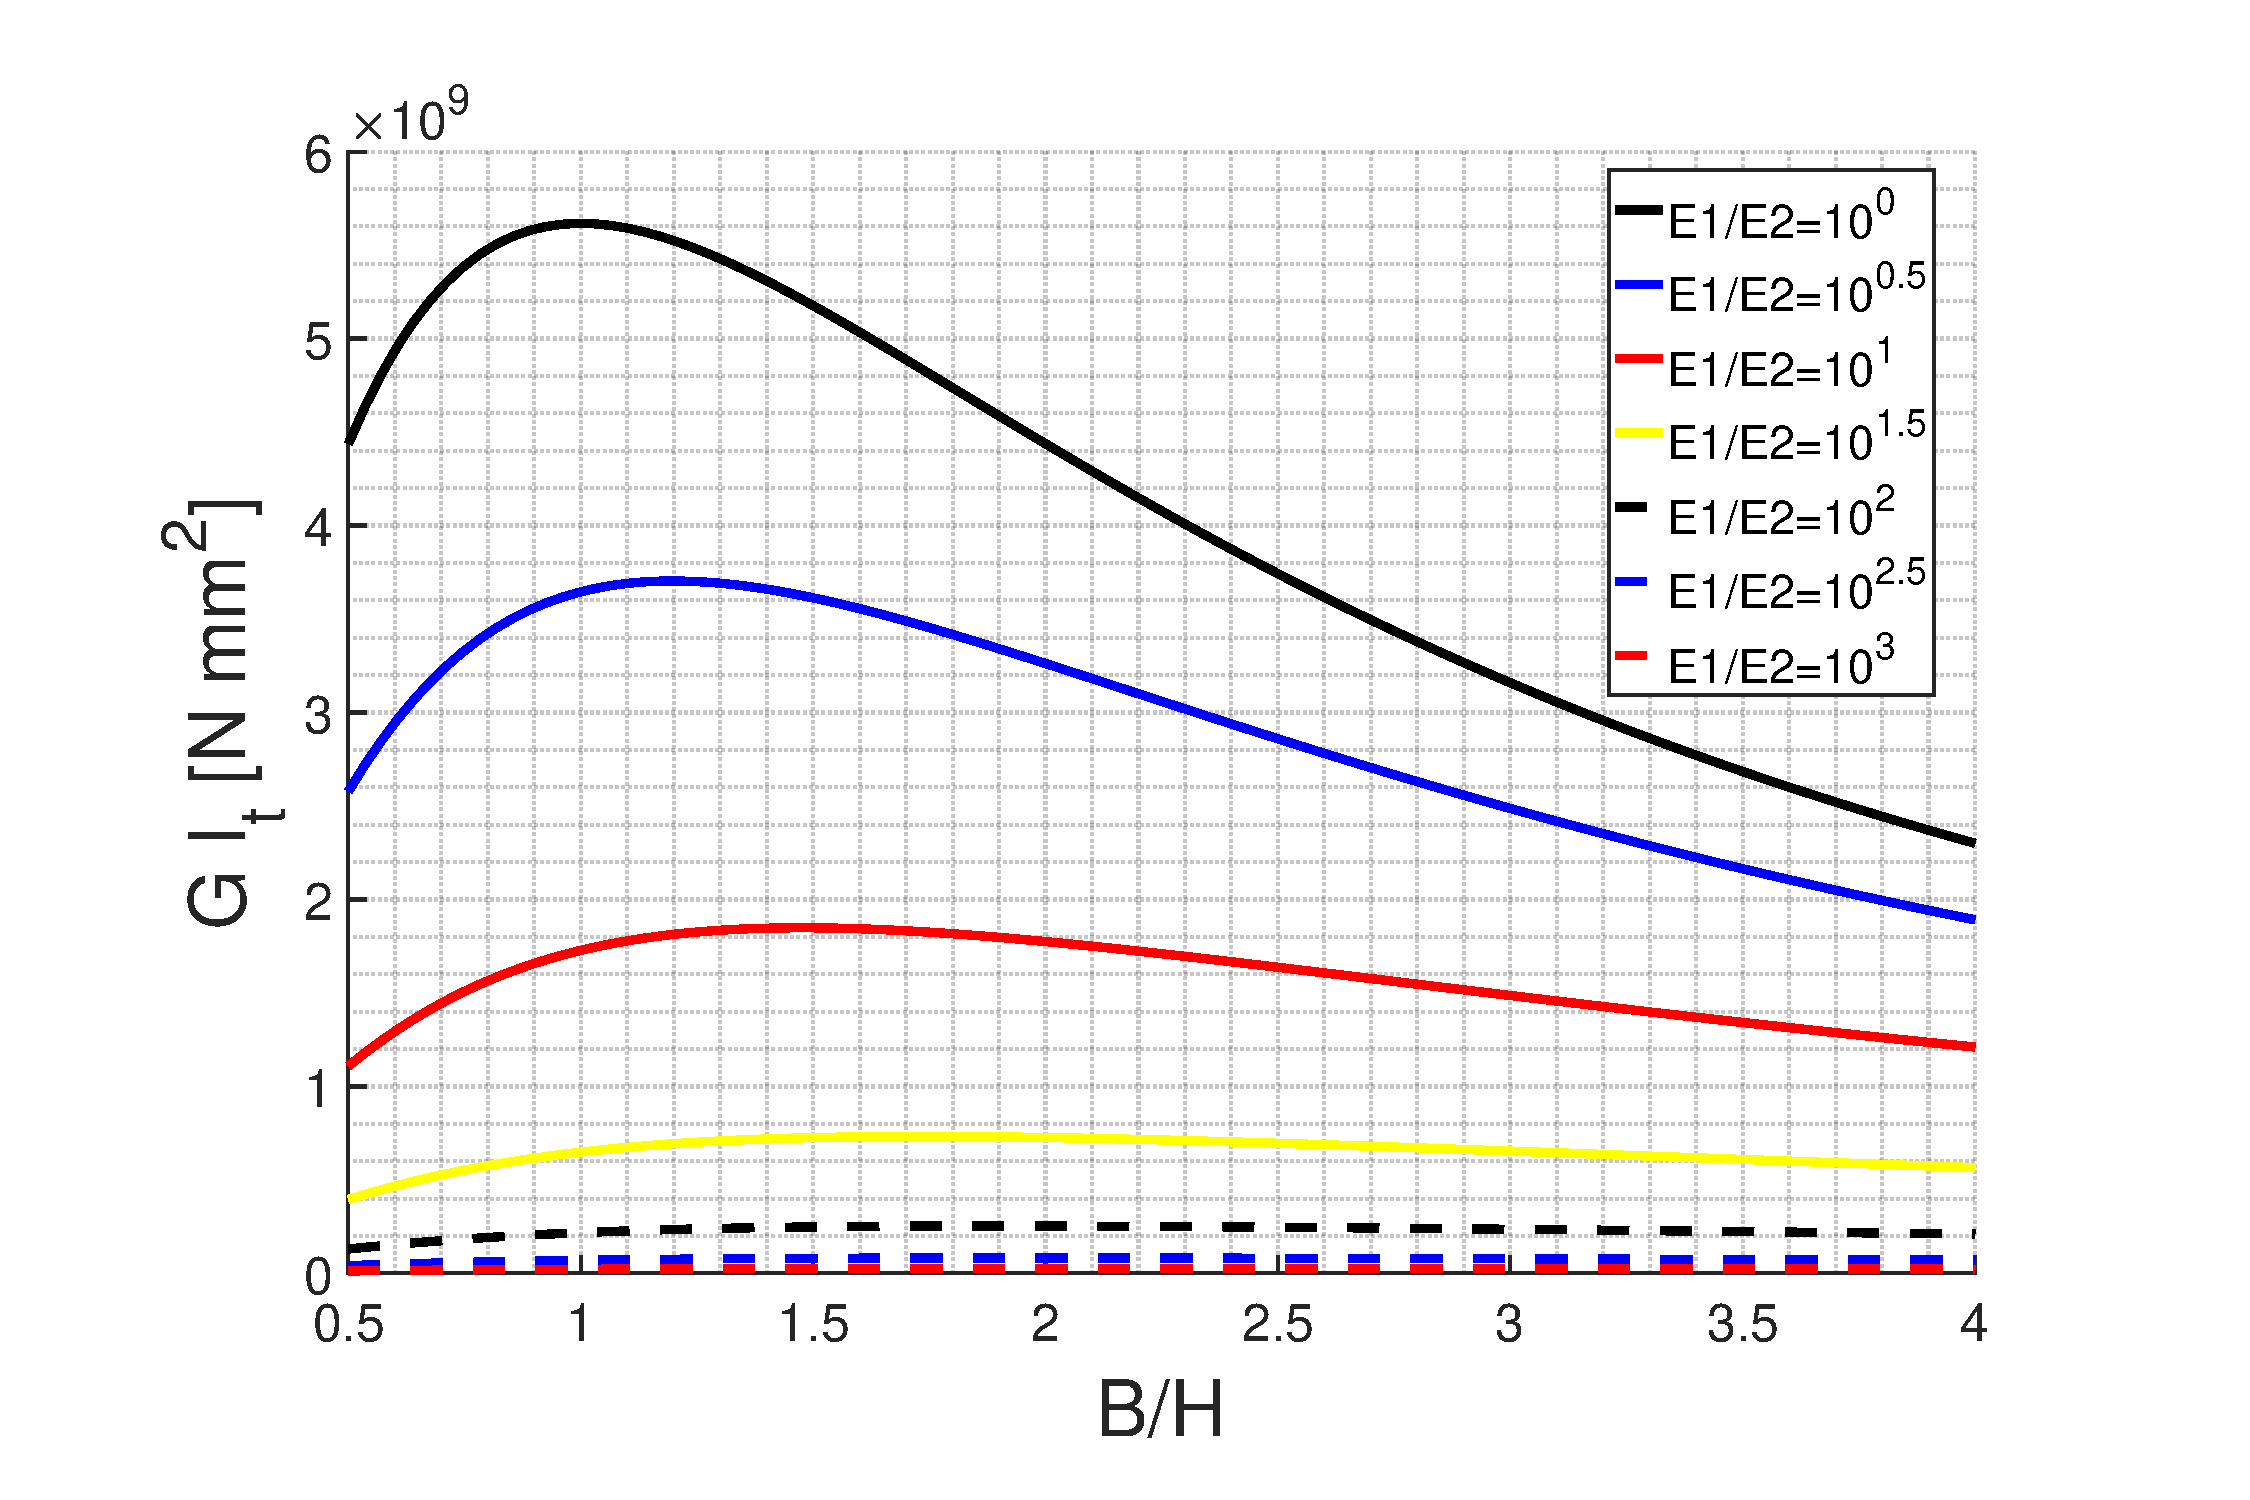
\includegraphics[width=0.8 \textwidth]{../../analytical/figures/GIt-E1overE2-BoverH}
  \caption[Influence of the cross-sectional aspect ratio $B/H$ on the torsional stiffness $GI_t$]{Influence of the cross-sectional aspect ratio $B/H$ on the torsional stiffness $GI_t$ is shown for various values of the stiffness ratio $E_1/E_2$ ranging from $10^0$ to $10^3$. }\label{fig:GIt-E1overE2-BoverH}
\end{figure}

\begin{figure}[!htpb] %Shear centre versus B/H
  \centering
  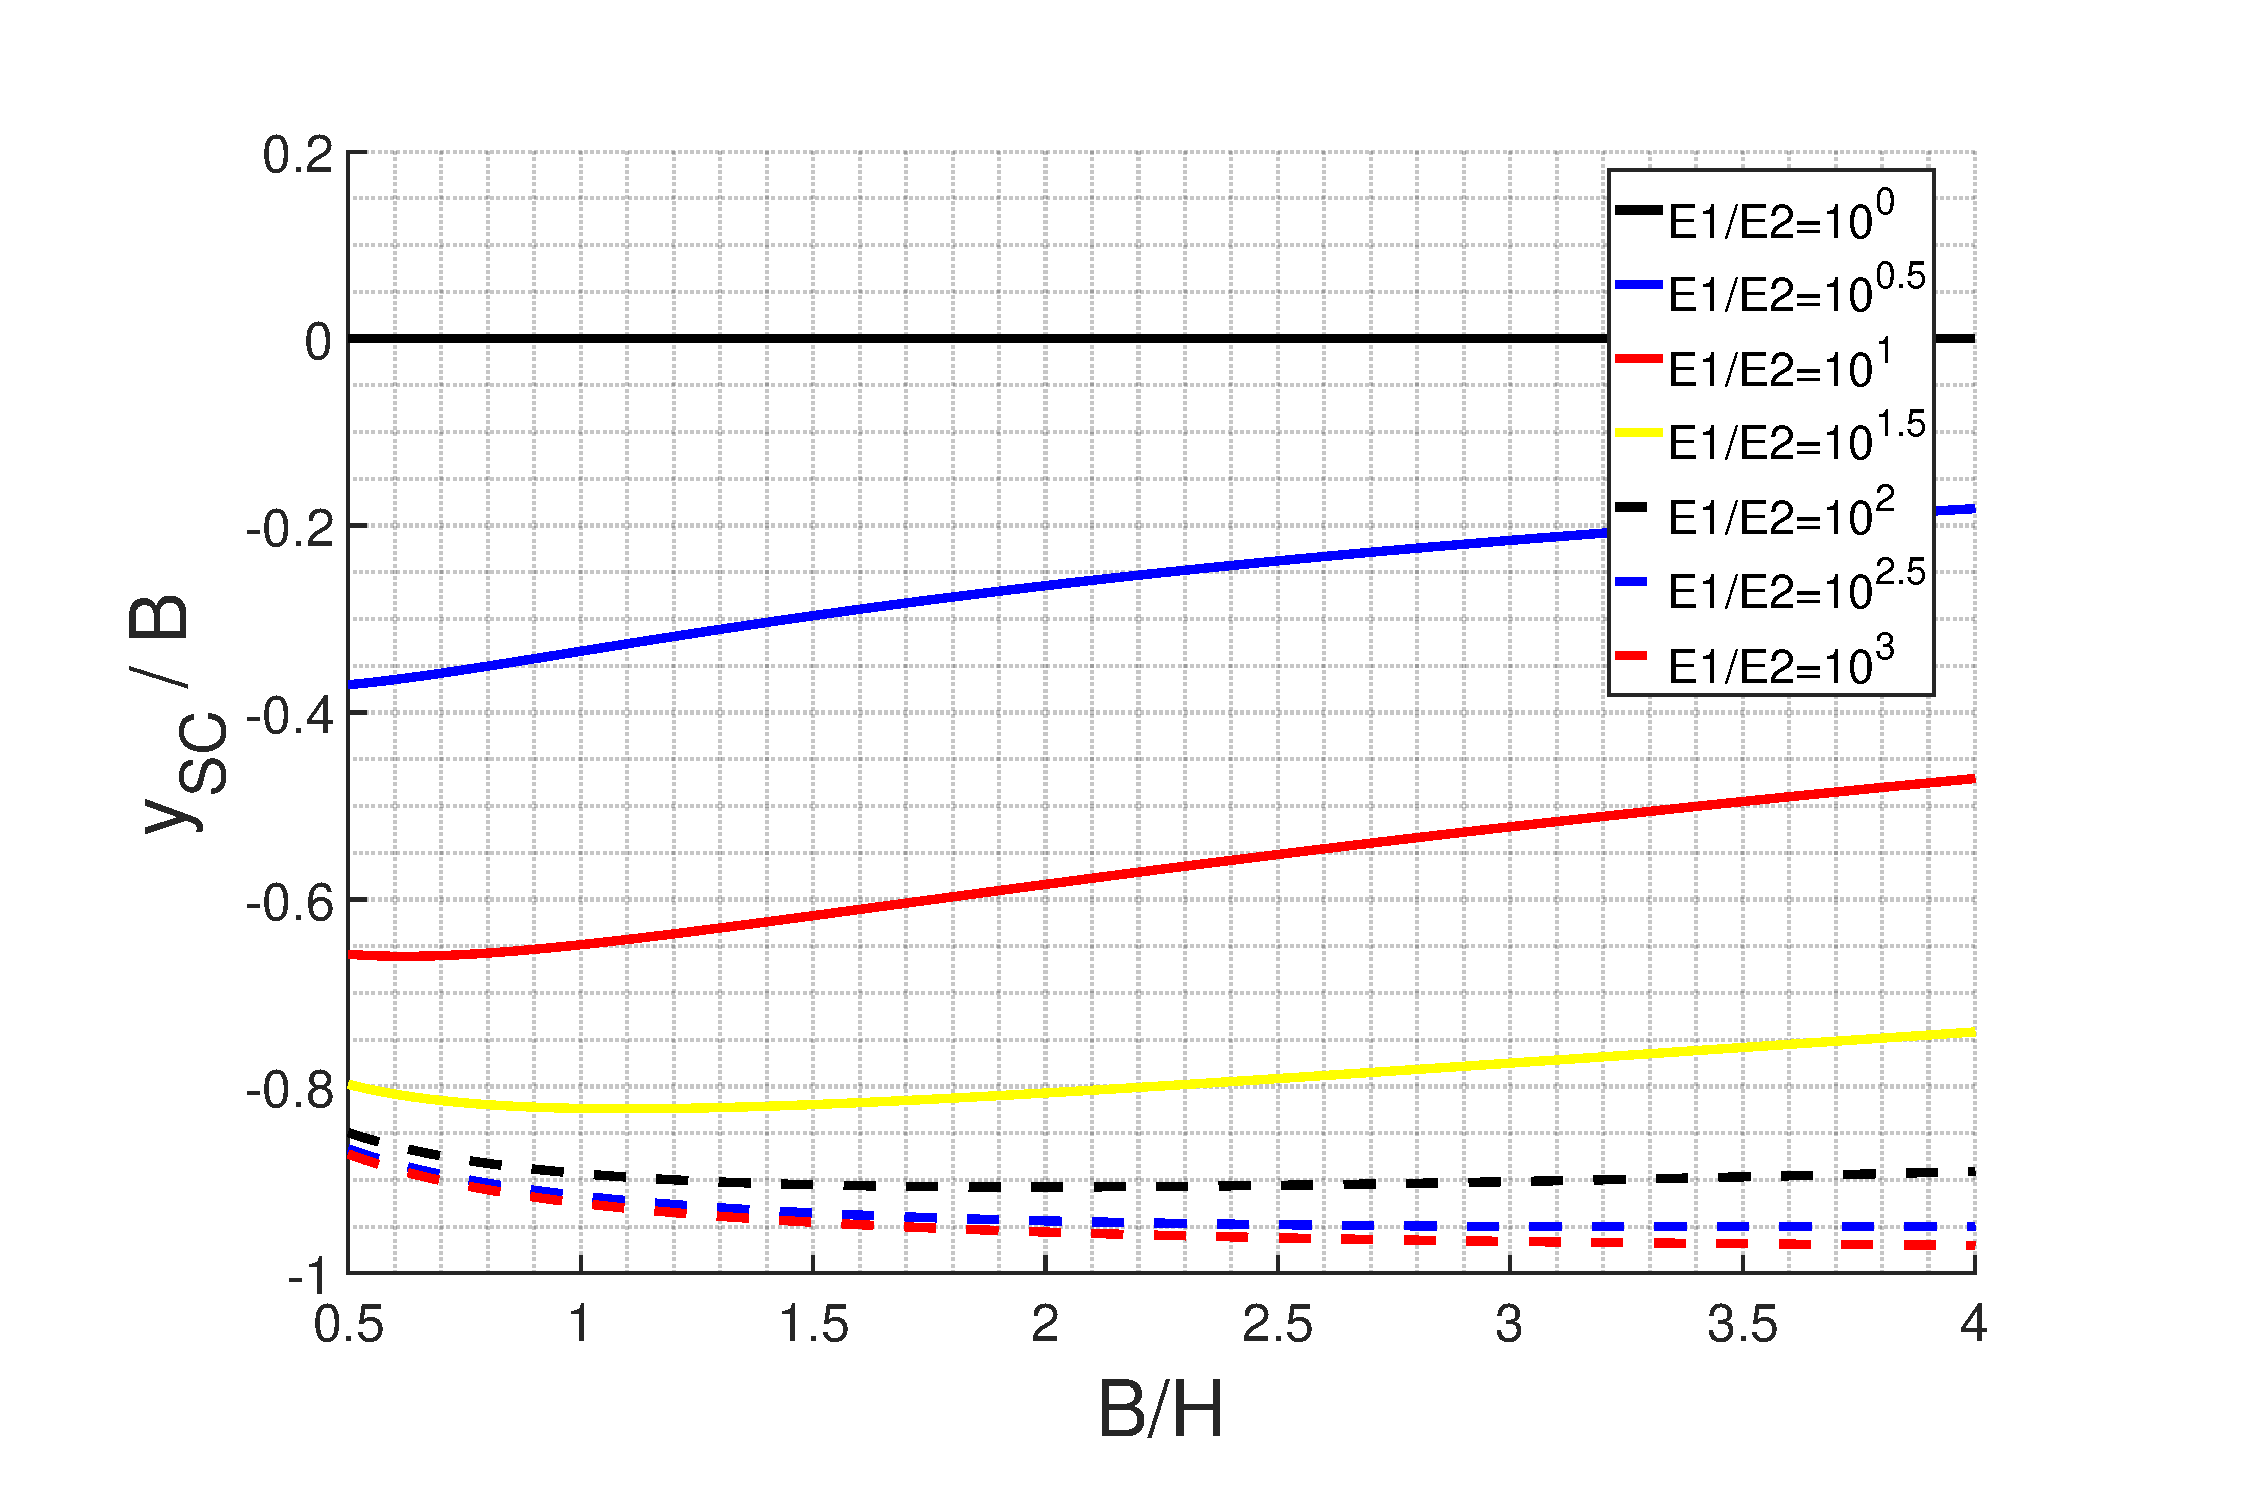
\includegraphics[width=0.8 \textwidth]{../../analytical/figures/SC-E1overE2-BoverH}
  \caption[Influence of the cross-sectional aspect ratio $B/H$ on the dimensionless shear centre position $y_{\mathrm{SC}}/B$]{Influence of the cross-sectional aspect ratio $B/H$ on the dimensionless shear centre position $y_{\mathrm{SC}}/B$ is shown for various values of the stiffness ratio $E_1/E_2$ ranging from $10^0$ to $10^3$. }\label{fig:SC-E1overE2-BoverH}
\end{figure}

\begin{figure}[!htpb] %E I_y = \Phi_y versus B/H
  \centering
  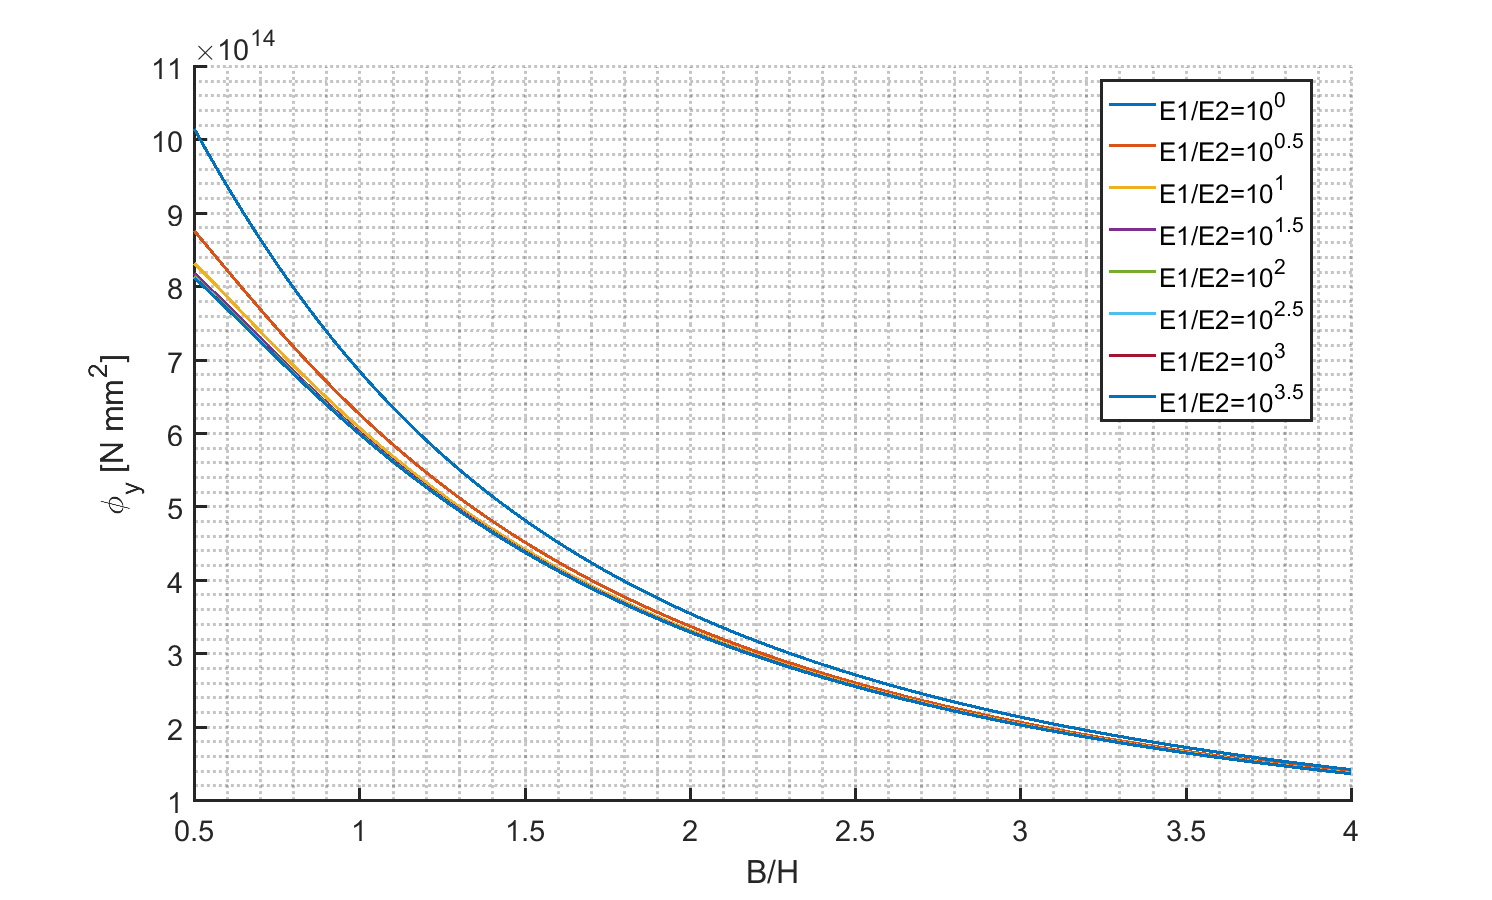
\includegraphics[width=0.8 \textwidth]{../../analytical/figures/EIy-E1overE2-BoverH}
  \caption[Influence of the cross-sectional aspect ratio $B/H$ on the flexural stiffness $EI_y$]{Influence of the cross-sectional aspect ratio $B/H$ on the flexural stiffness $EI_y = \Phi_y$ is shown for various values of the stiffness ratio $E_1/E_2$ ranging from $10^0$ to $10^3$. }\label{fig:EIy-E1overE2-BoverH}
\end{figure}

\begin{figure}[!htpb] %w_0,tip / Q versus B/H, deflection compliance
  \centering
  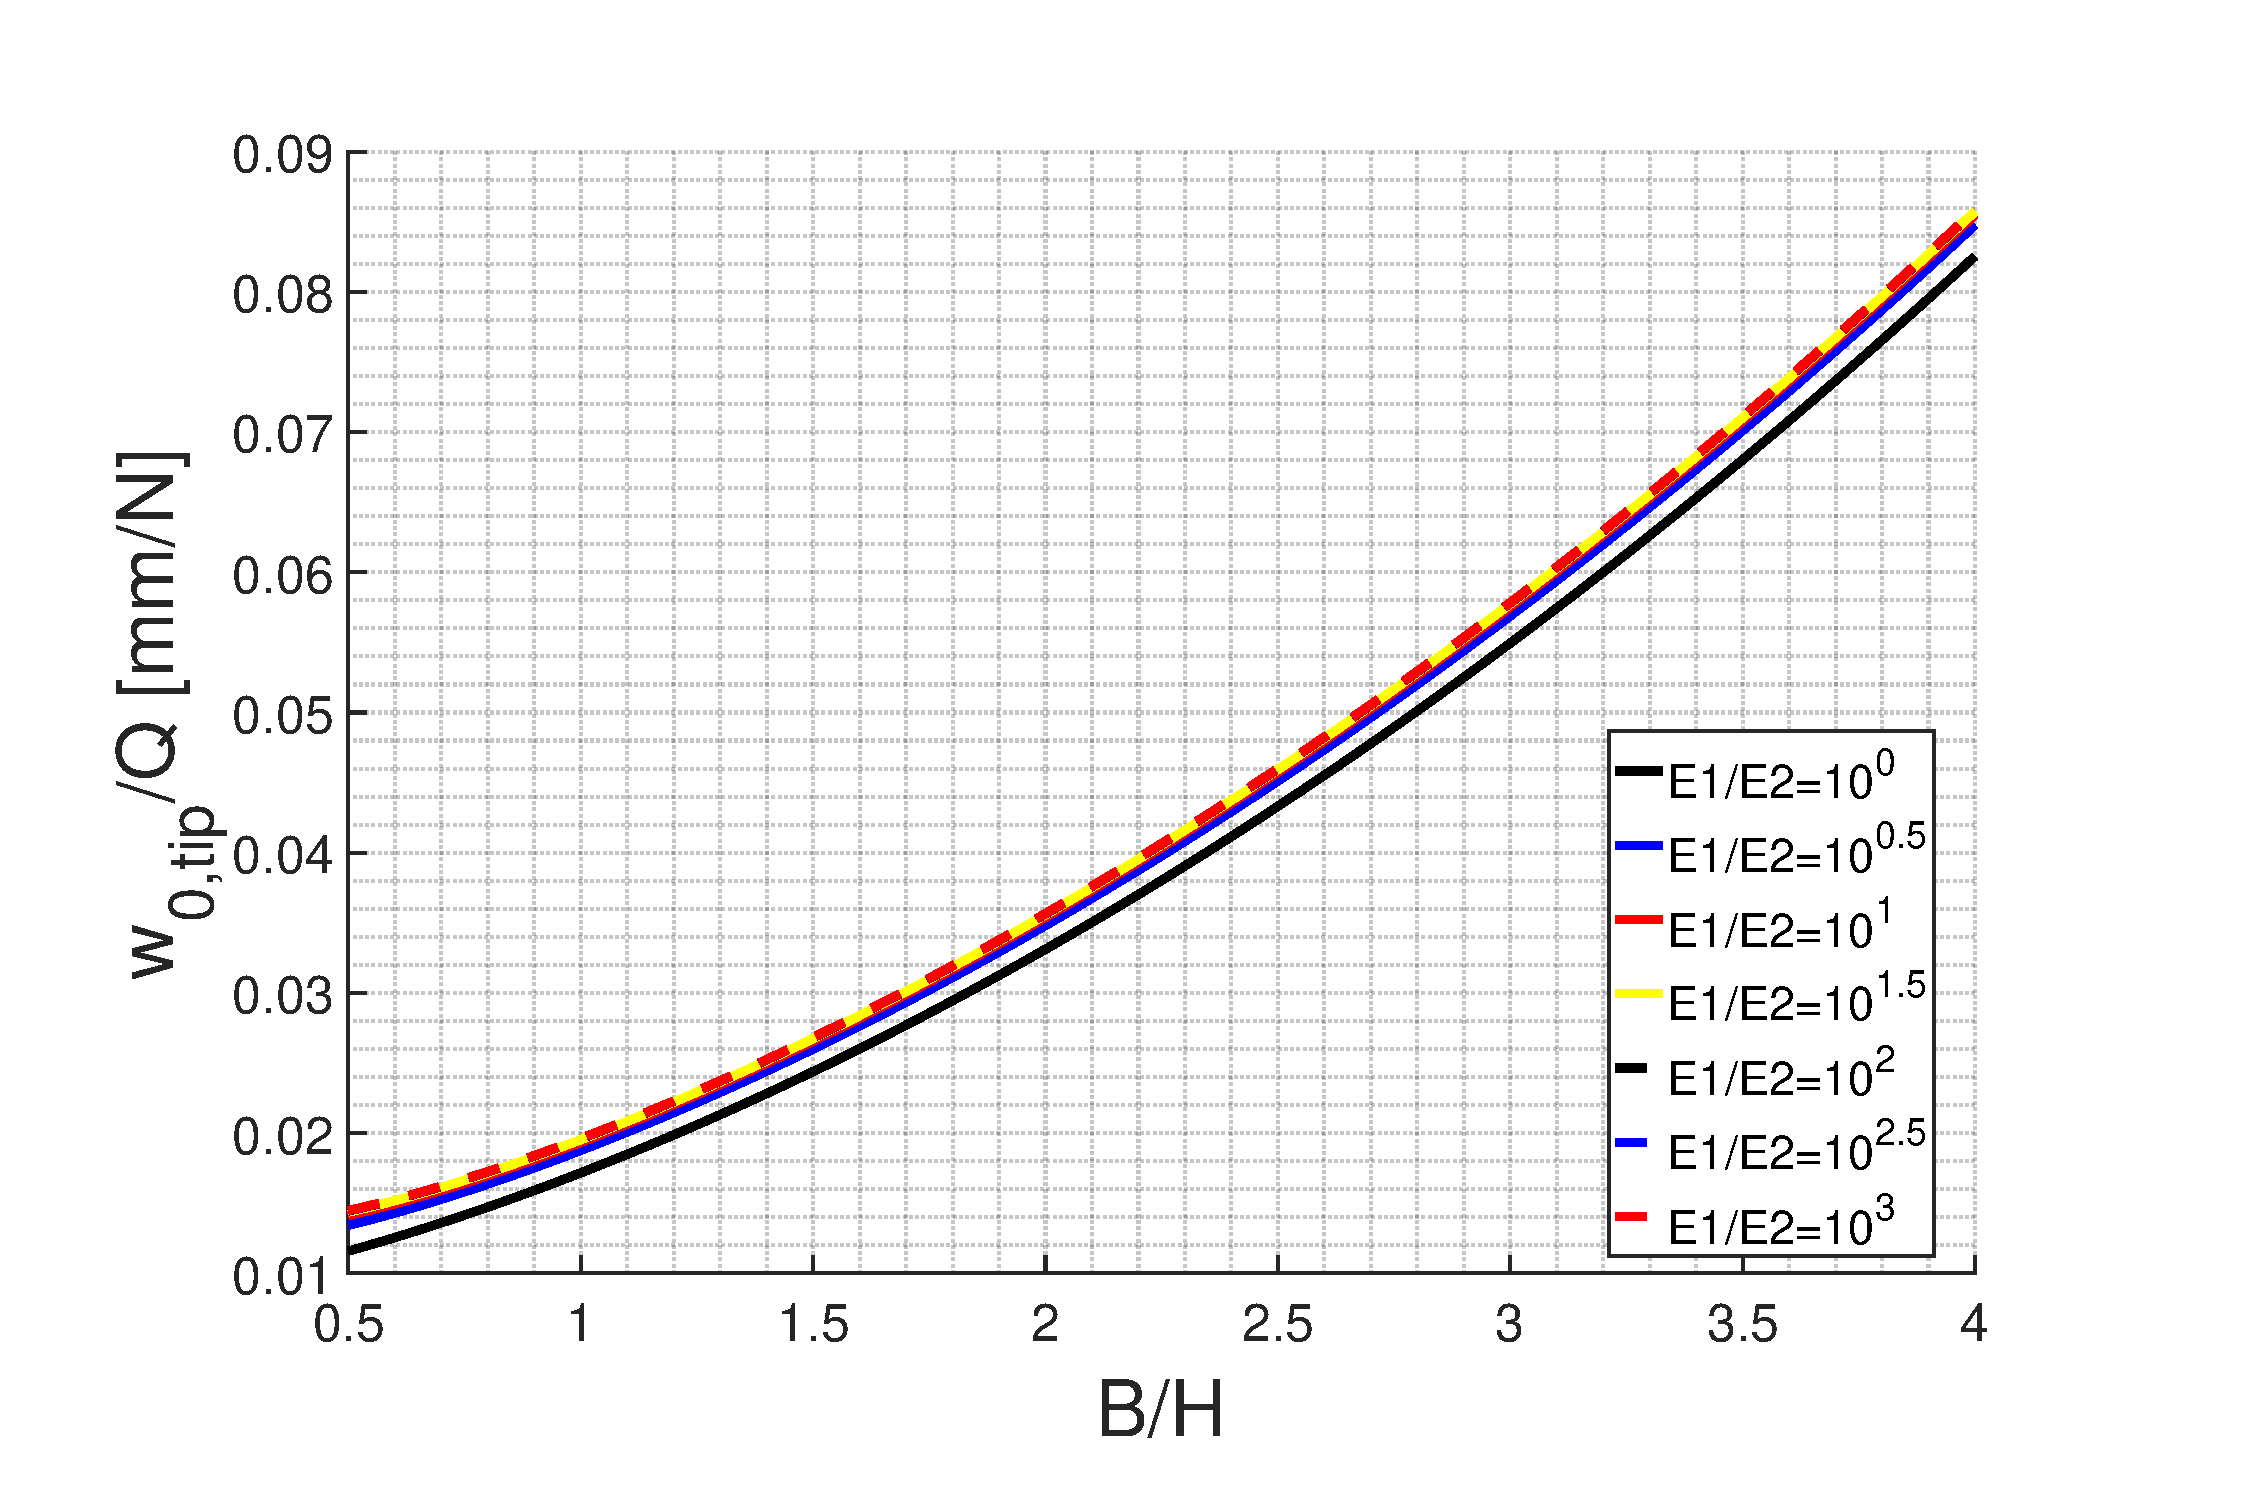
\includegraphics[width=0.8 \textwidth]{../../analytical/figures/woverQ-E1overE2-BoverH}
  \caption[Influence of the cross-sectional aspect ratio $B/H$ on the deflection compliance]{Influence of the cross-sectional aspect ratio $B/H$ on the deflection compliance $w_{\mathrm{0,tip}} / Q$ is shown for various values of the stiffness ratio $E_1/E_2$ ranging from $10^0$ to $10^3$. }\label{fig:woverQ-E1overE2-BoverH}
\end{figure}

\begin{figure}[!htpb] %\phi_tip / Q versus B/H, torsional compliance
  \centering
  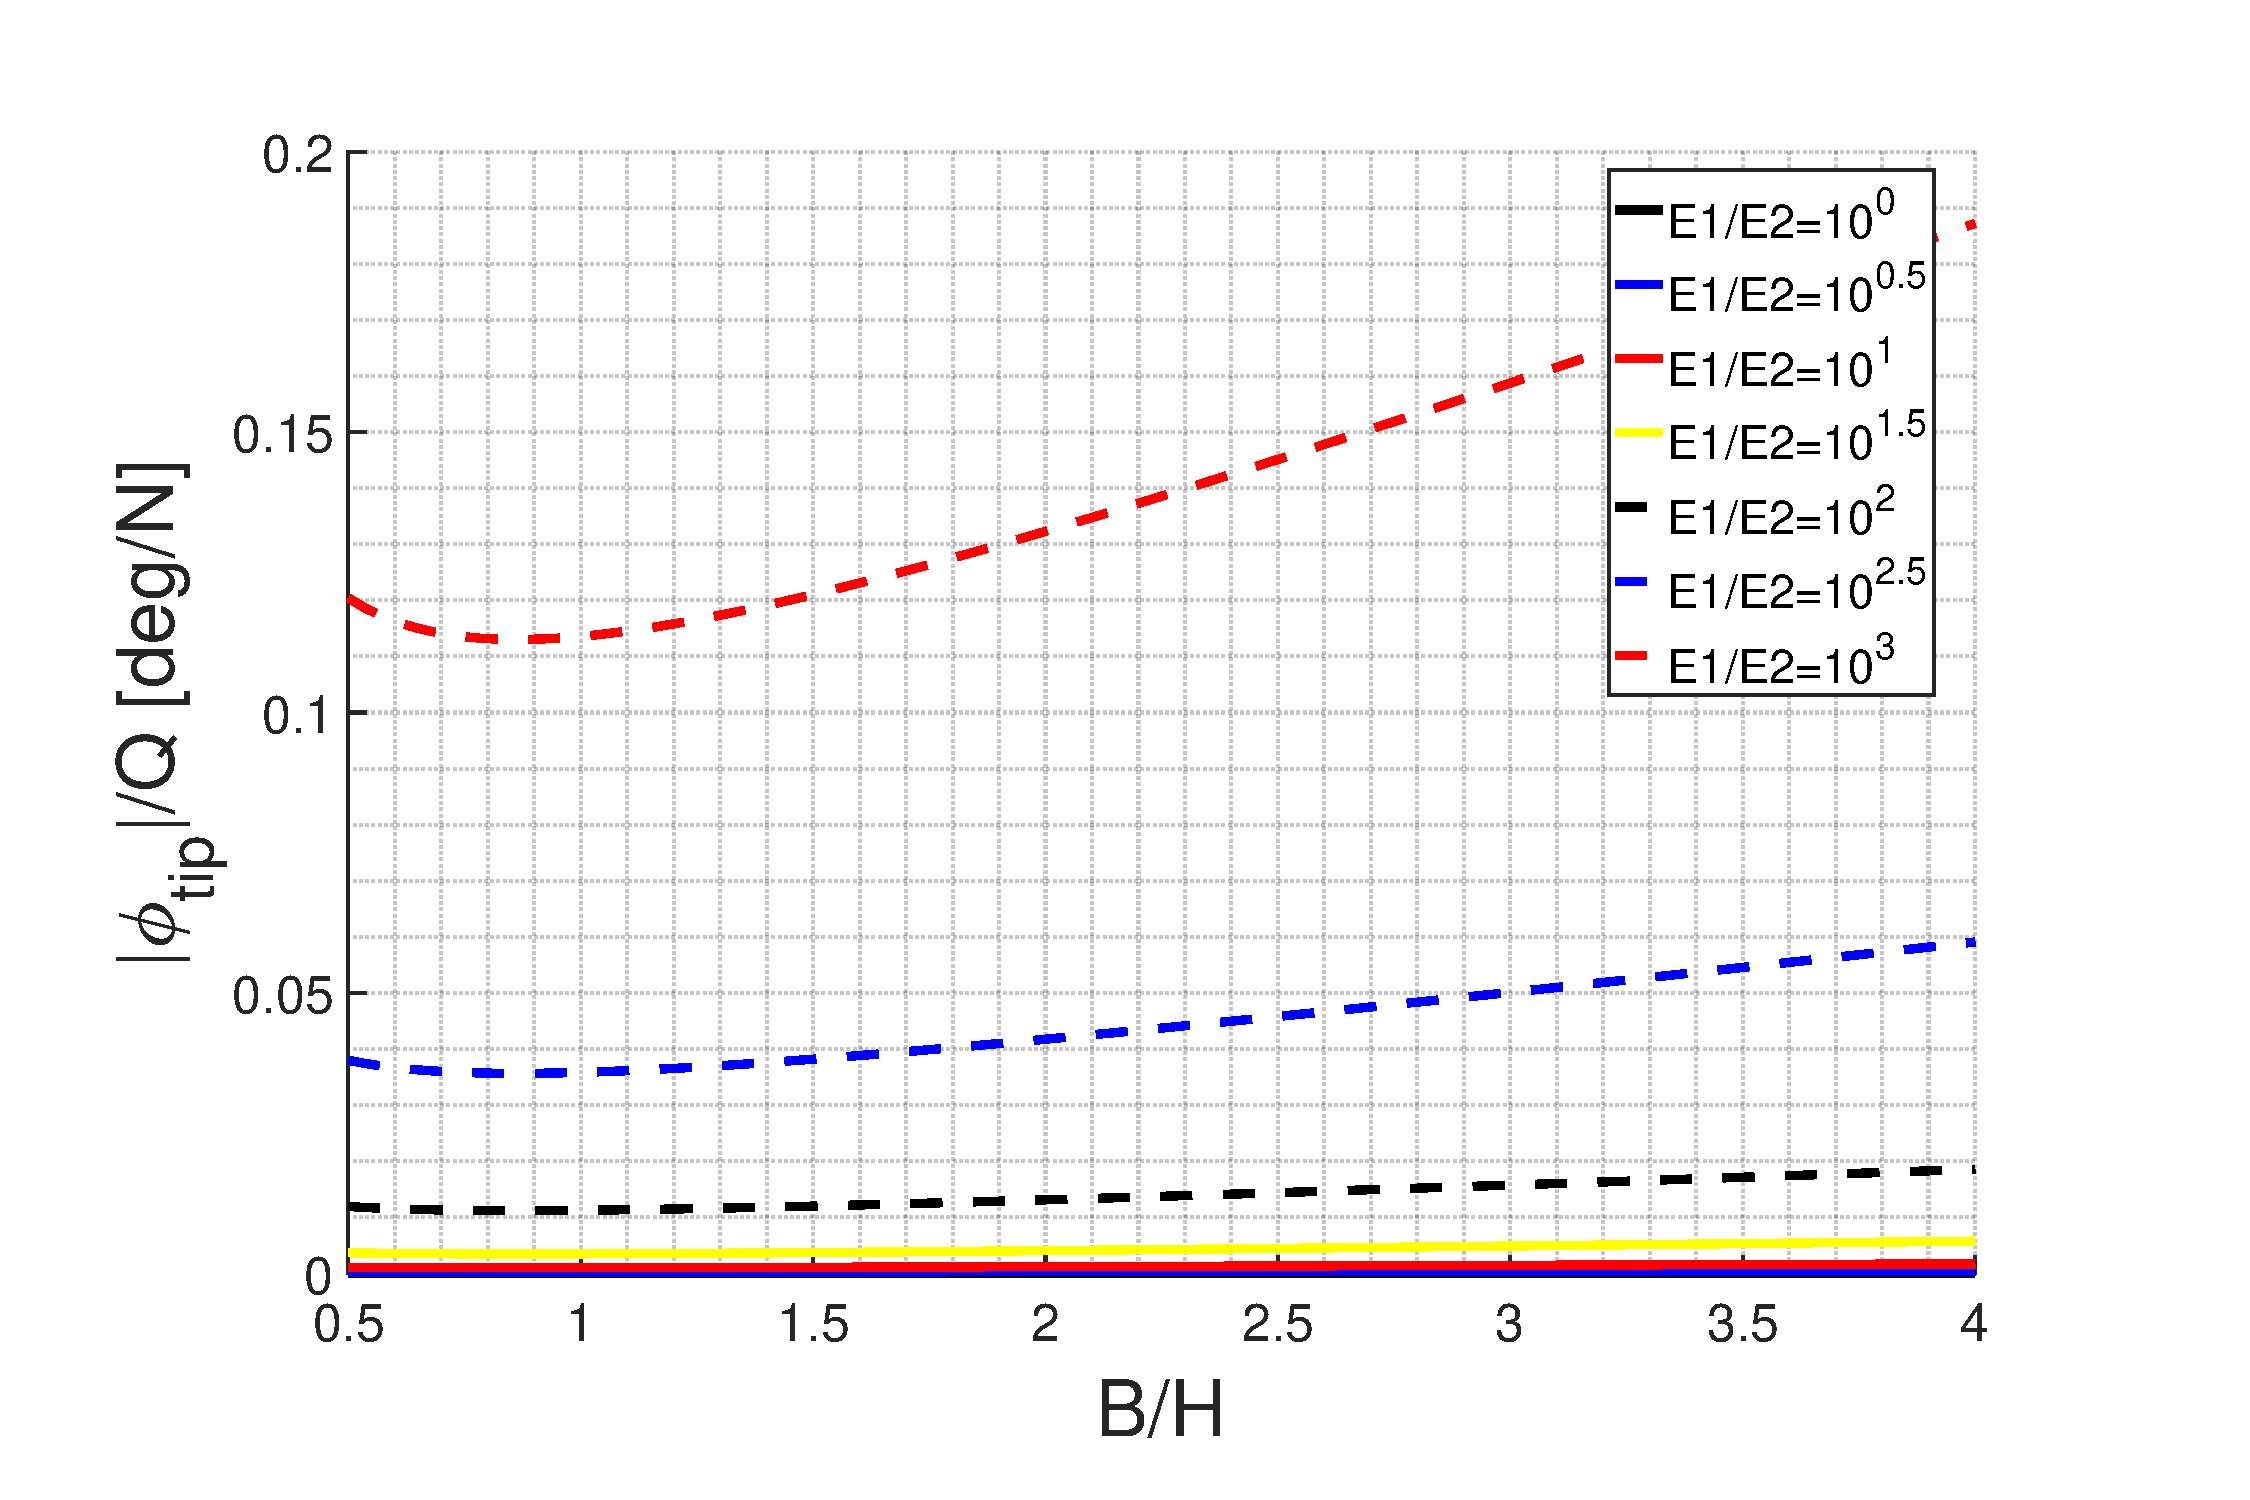
\includegraphics[width=0.8 \textwidth]{../../analytical/figures/phioverQ-E1overE2-BoverH}
  \caption[Influence of the cross-sectional aspect ratio $B/H$ on the torsional compliance]{Influence of the cross-sectional aspect ratio $B/H$ on the torsional compliance $|\phi_{\mathrm{tip}}| / Q$ is shown for various values of the stiffness ratio $E_1/E_2$ ranging from $10^0$ to $10^3$. }\label{fig:phioverQ-E1overE2-BoverH}
\end{figure}

%%%% Figures variation of t2/t1
\begin{figure}[!htpb] %G I_t versus t2/t1
  \centering
  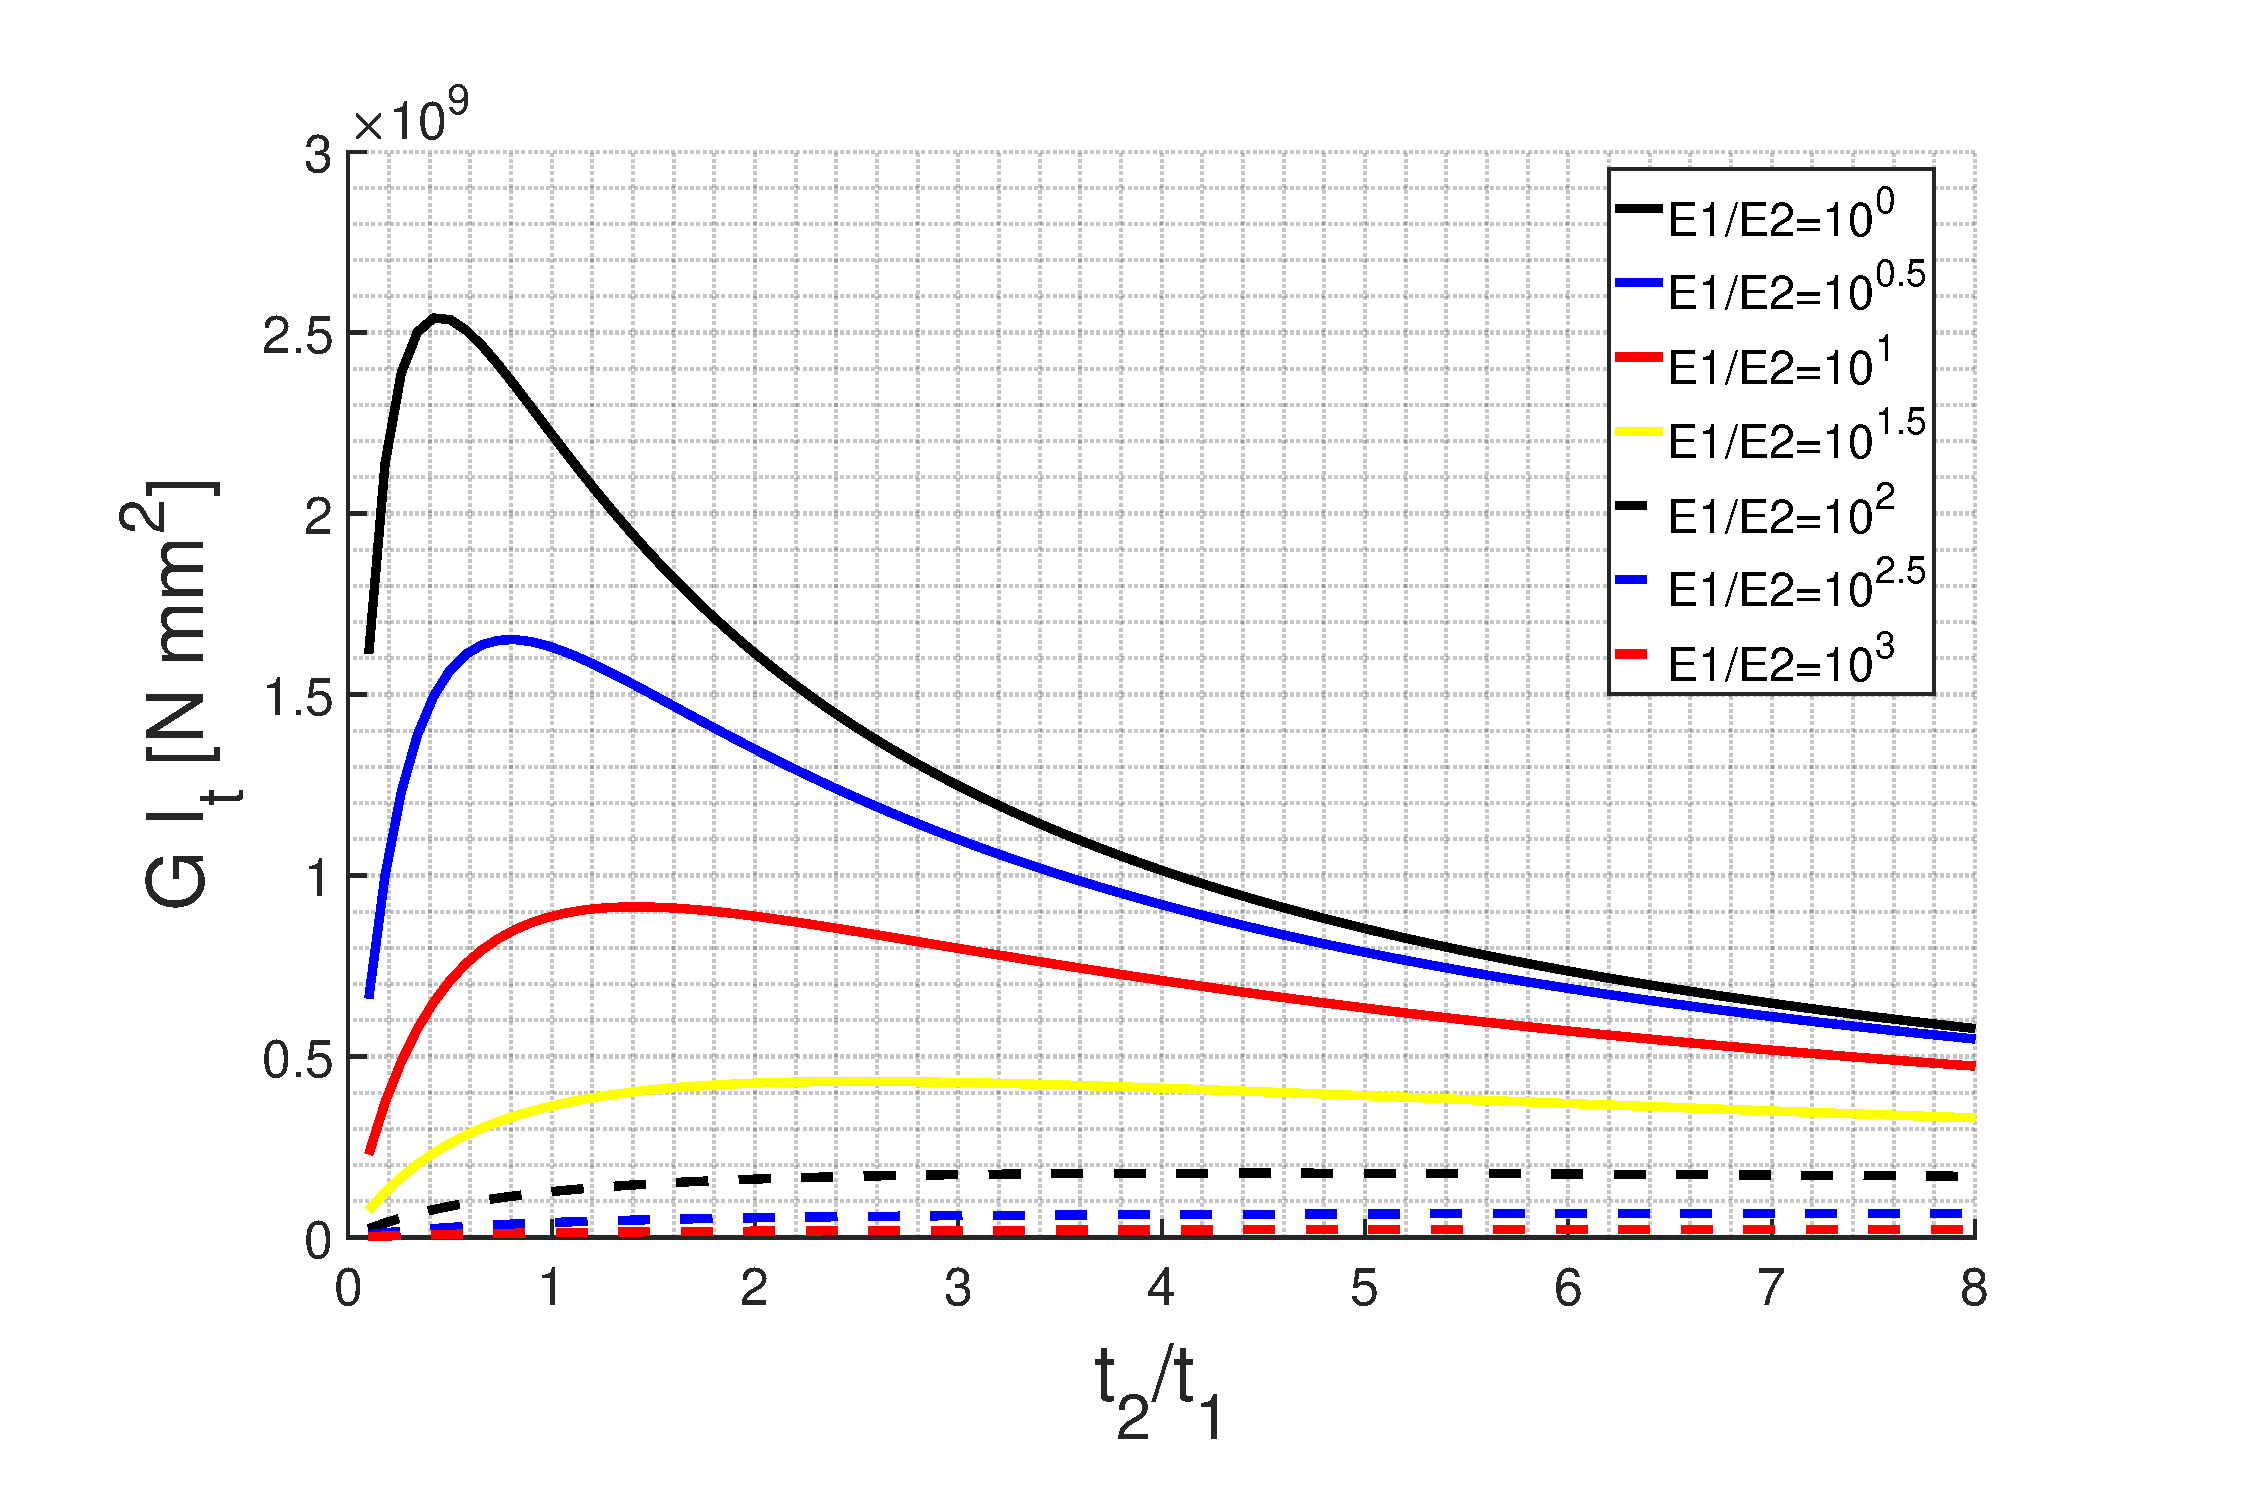
\includegraphics[width=0.8 \textwidth]{../../analytical/figures/GIt-E1overE2-t2overt1}
  \caption[Influence of the wall thickness ratio $t_2/t_1$ on the torsional stiffness $GI_t$]{Influence of the wall thickness ratio $t_2/t_1$ on the torsional stiffness $GI_t$ shown for various values of the stiffness ratio $E_1/E_2$ ranging from $10^0$ to $10^3$. }\label{fig:GIt-E1overE2-t2overt1}
\end{figure}

\begin{figure}[!htpb] %Shear centre versus t2/t1
  \centering
  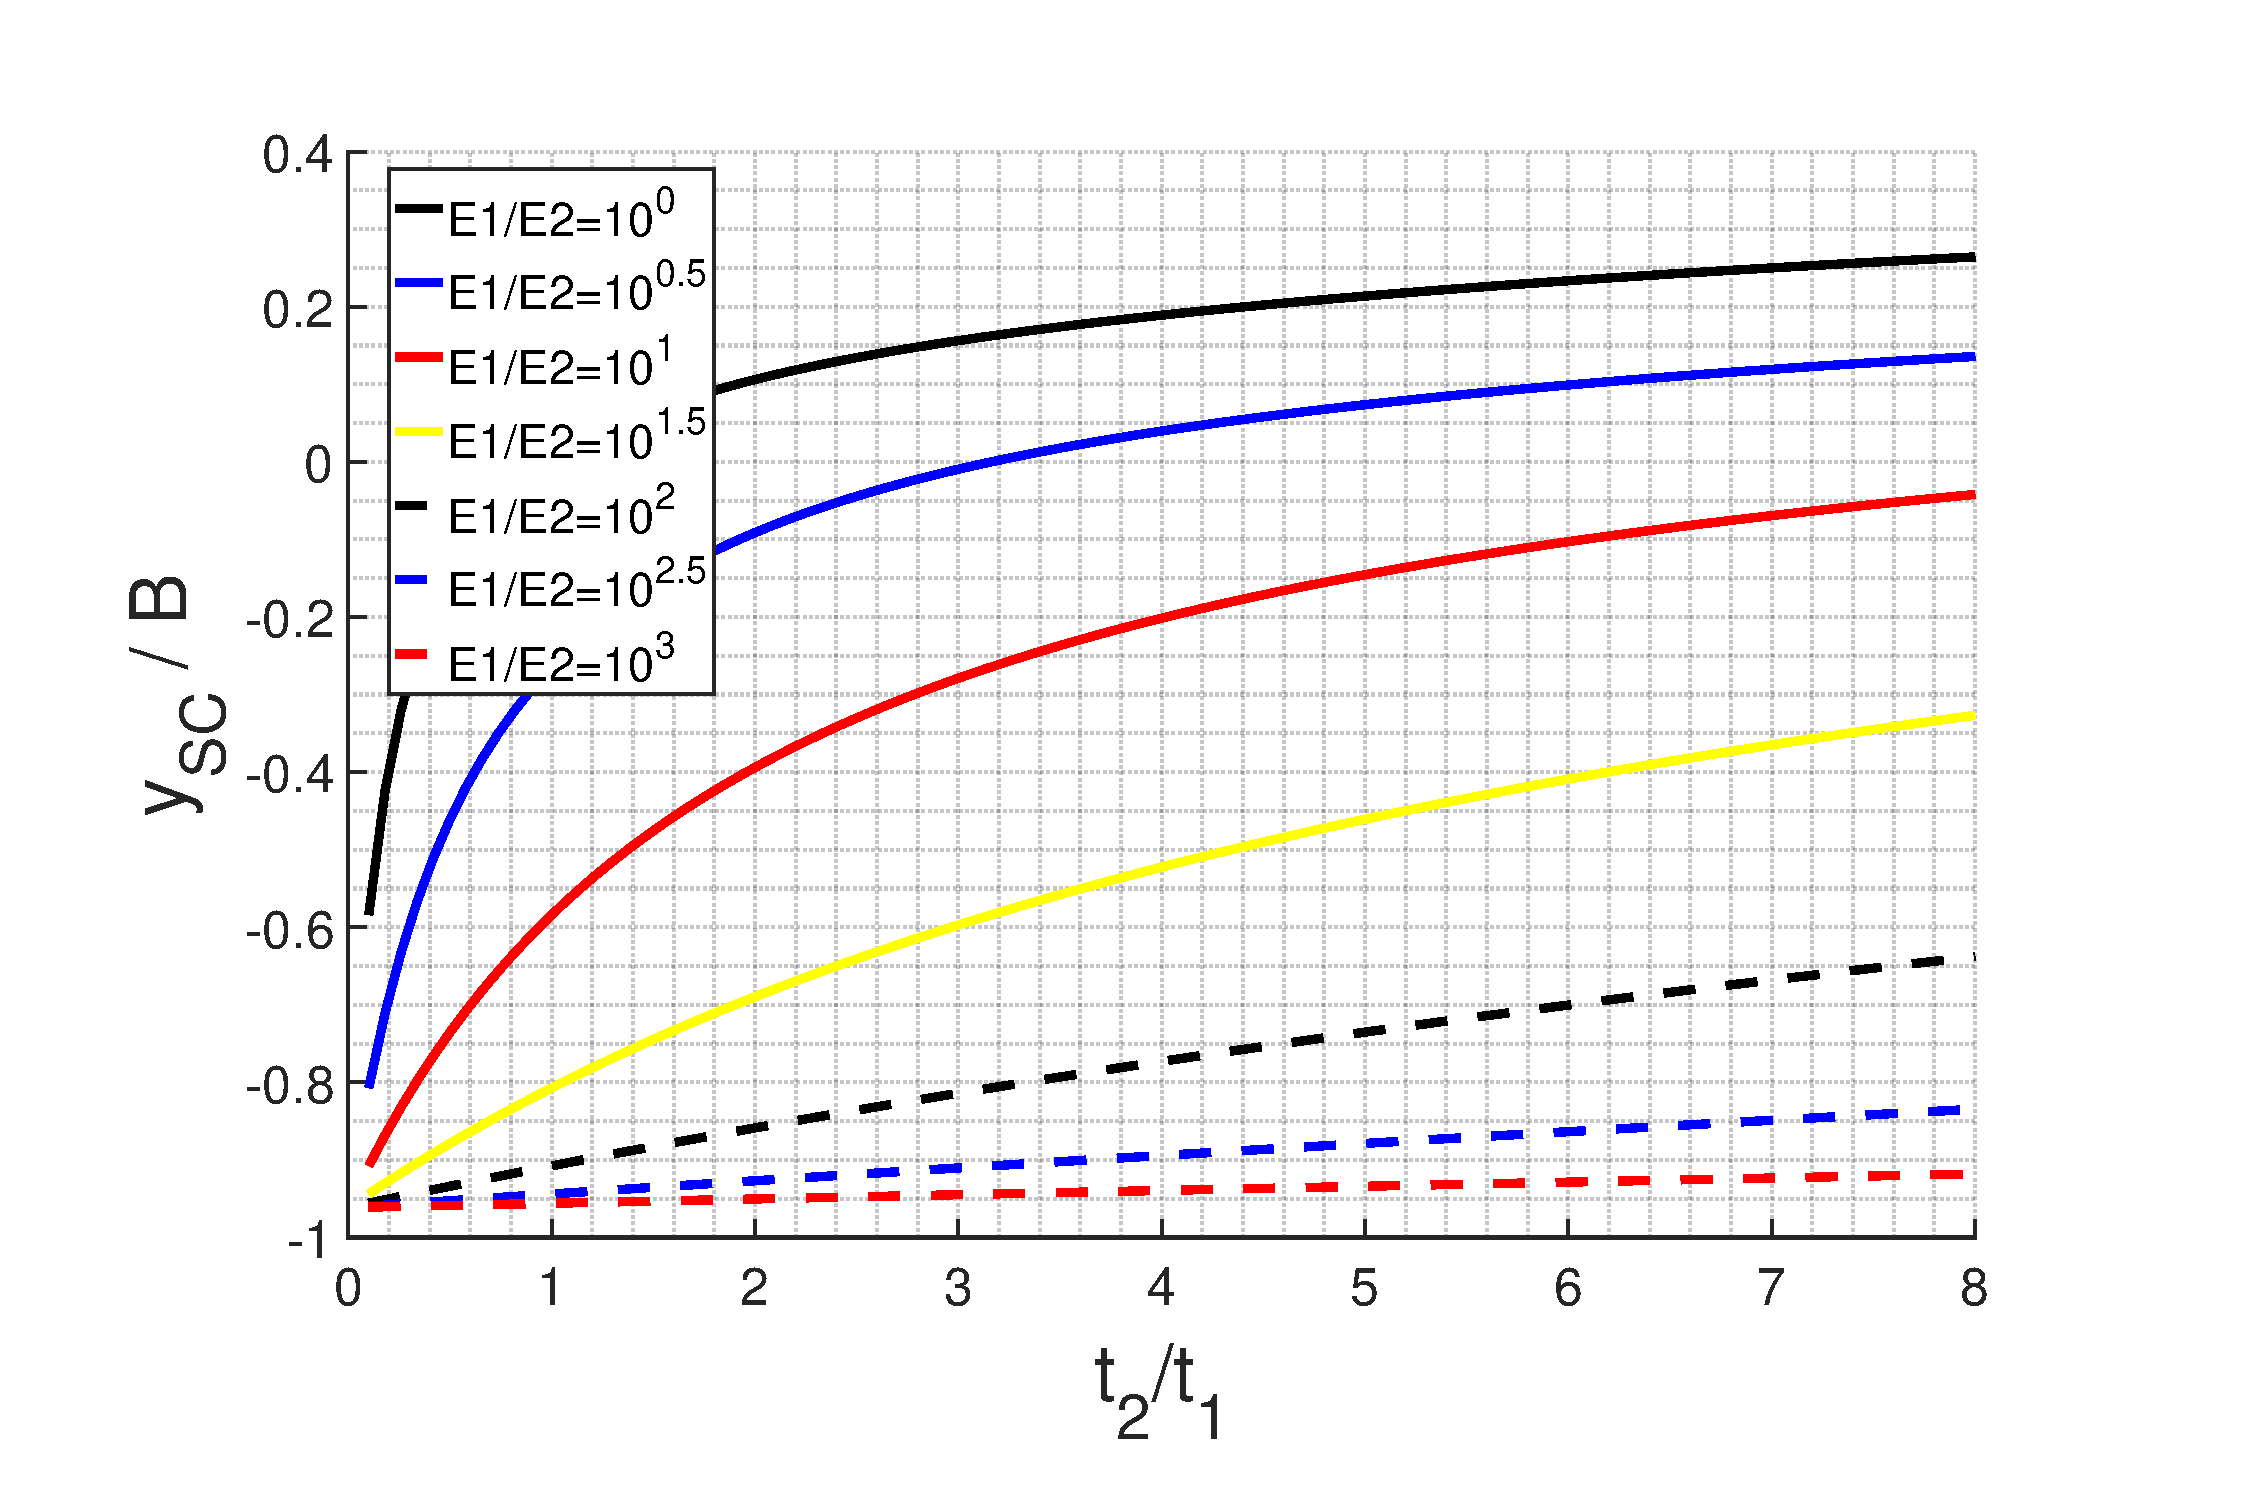
\includegraphics[width=0.8 \textwidth]{../../analytical/figures/SC-E1overE2-t2overt1}
  \caption[Influence of the wall thickness ratio $t_2/t_1$ on the dimensionless shear centre position $y_{\mathrm{SC}}/B$]{Influence of the wall thickness ratio $t_2/t_1$ on the dimensionless shear centre position $y_{\mathrm{SC}}/B$ shown for various values of the stiffness ratio $E_1/E_2$ ranging from $10^0$ to $10^3$. }\label{fig:SC-E1overE2-t2overt1}
\end{figure}

\begin{figure}[!htpb] %E I_y = \Phi_y versus t2/t1
  \centering
  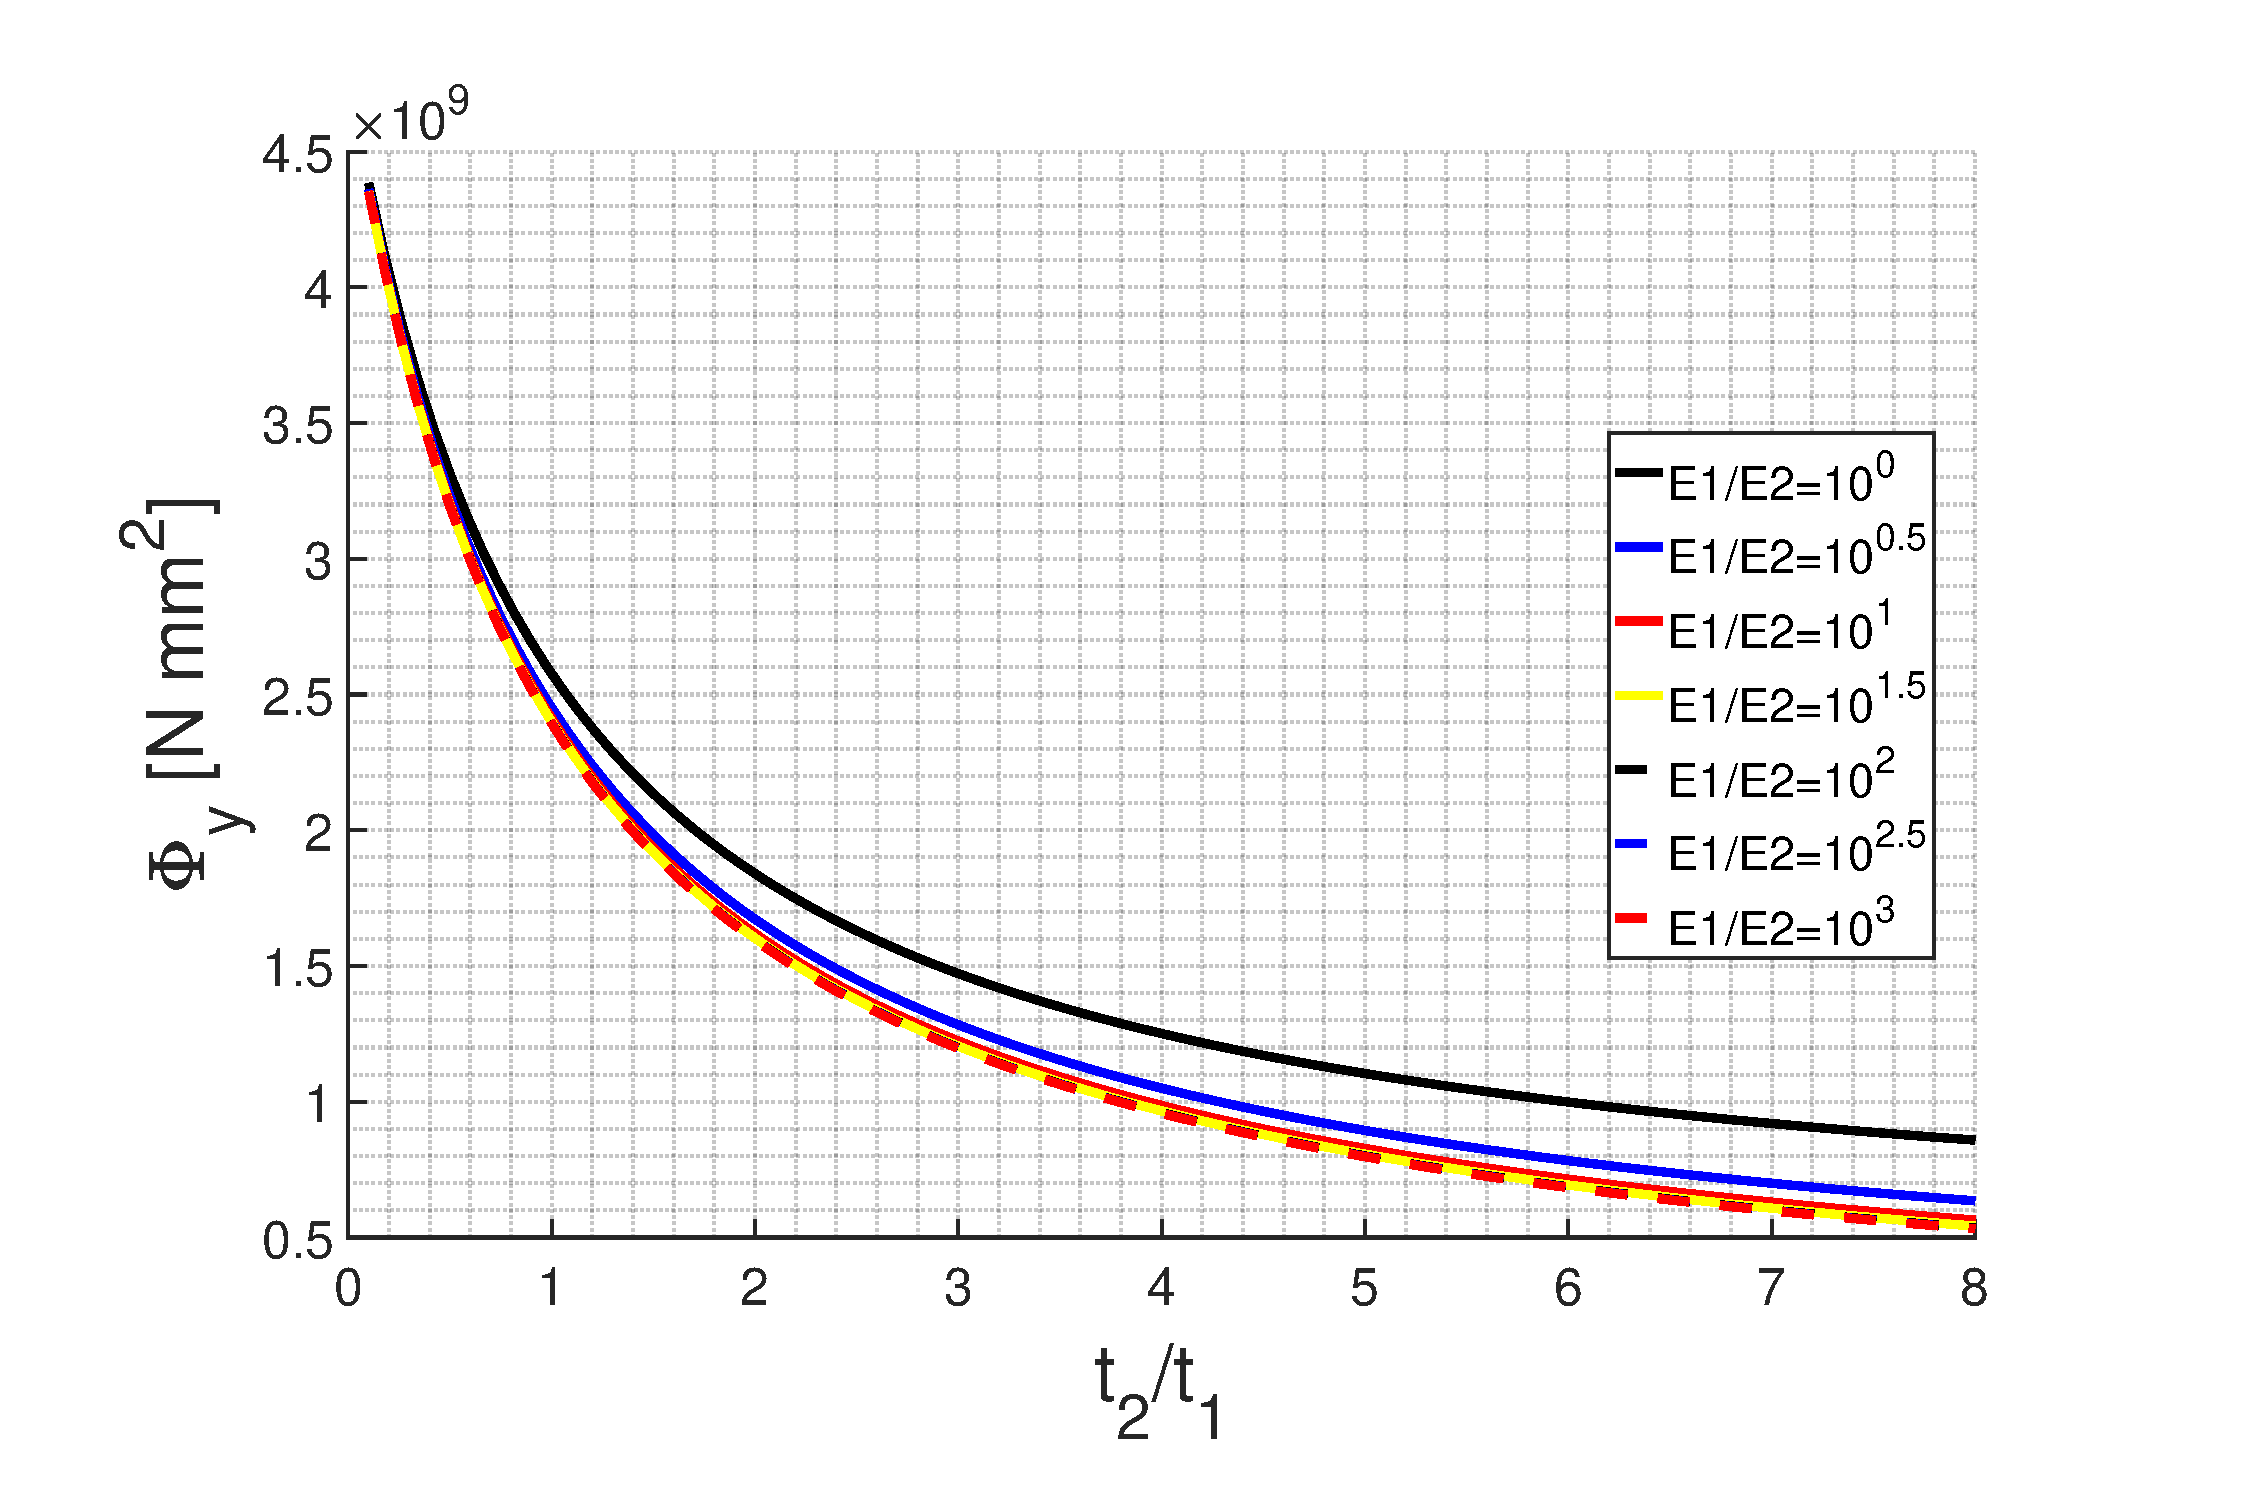
\includegraphics[width=0.8 \textwidth]{../../analytical/figures/EIy-E1overE2-t2overt1}
  \caption[Influence of the wall thickness ratio $t_2/t_1$ on the flexural stiffness $EI_y$]{Influence of the wall thickness ratio $t_2/t_1$ on the flexural stiffness $EI_y = \Phi_y$ shown for various values of the stiffness ratio $E_1/E_2$ ranging from $10^0$ to $10^3$. }\label{fig:EIy-E1overE2-t2overt1}
\end{figure}

\begin{figure}[!htpb] %w_0,tip / Q versus t2/t1, deflection compliance
  \centering
  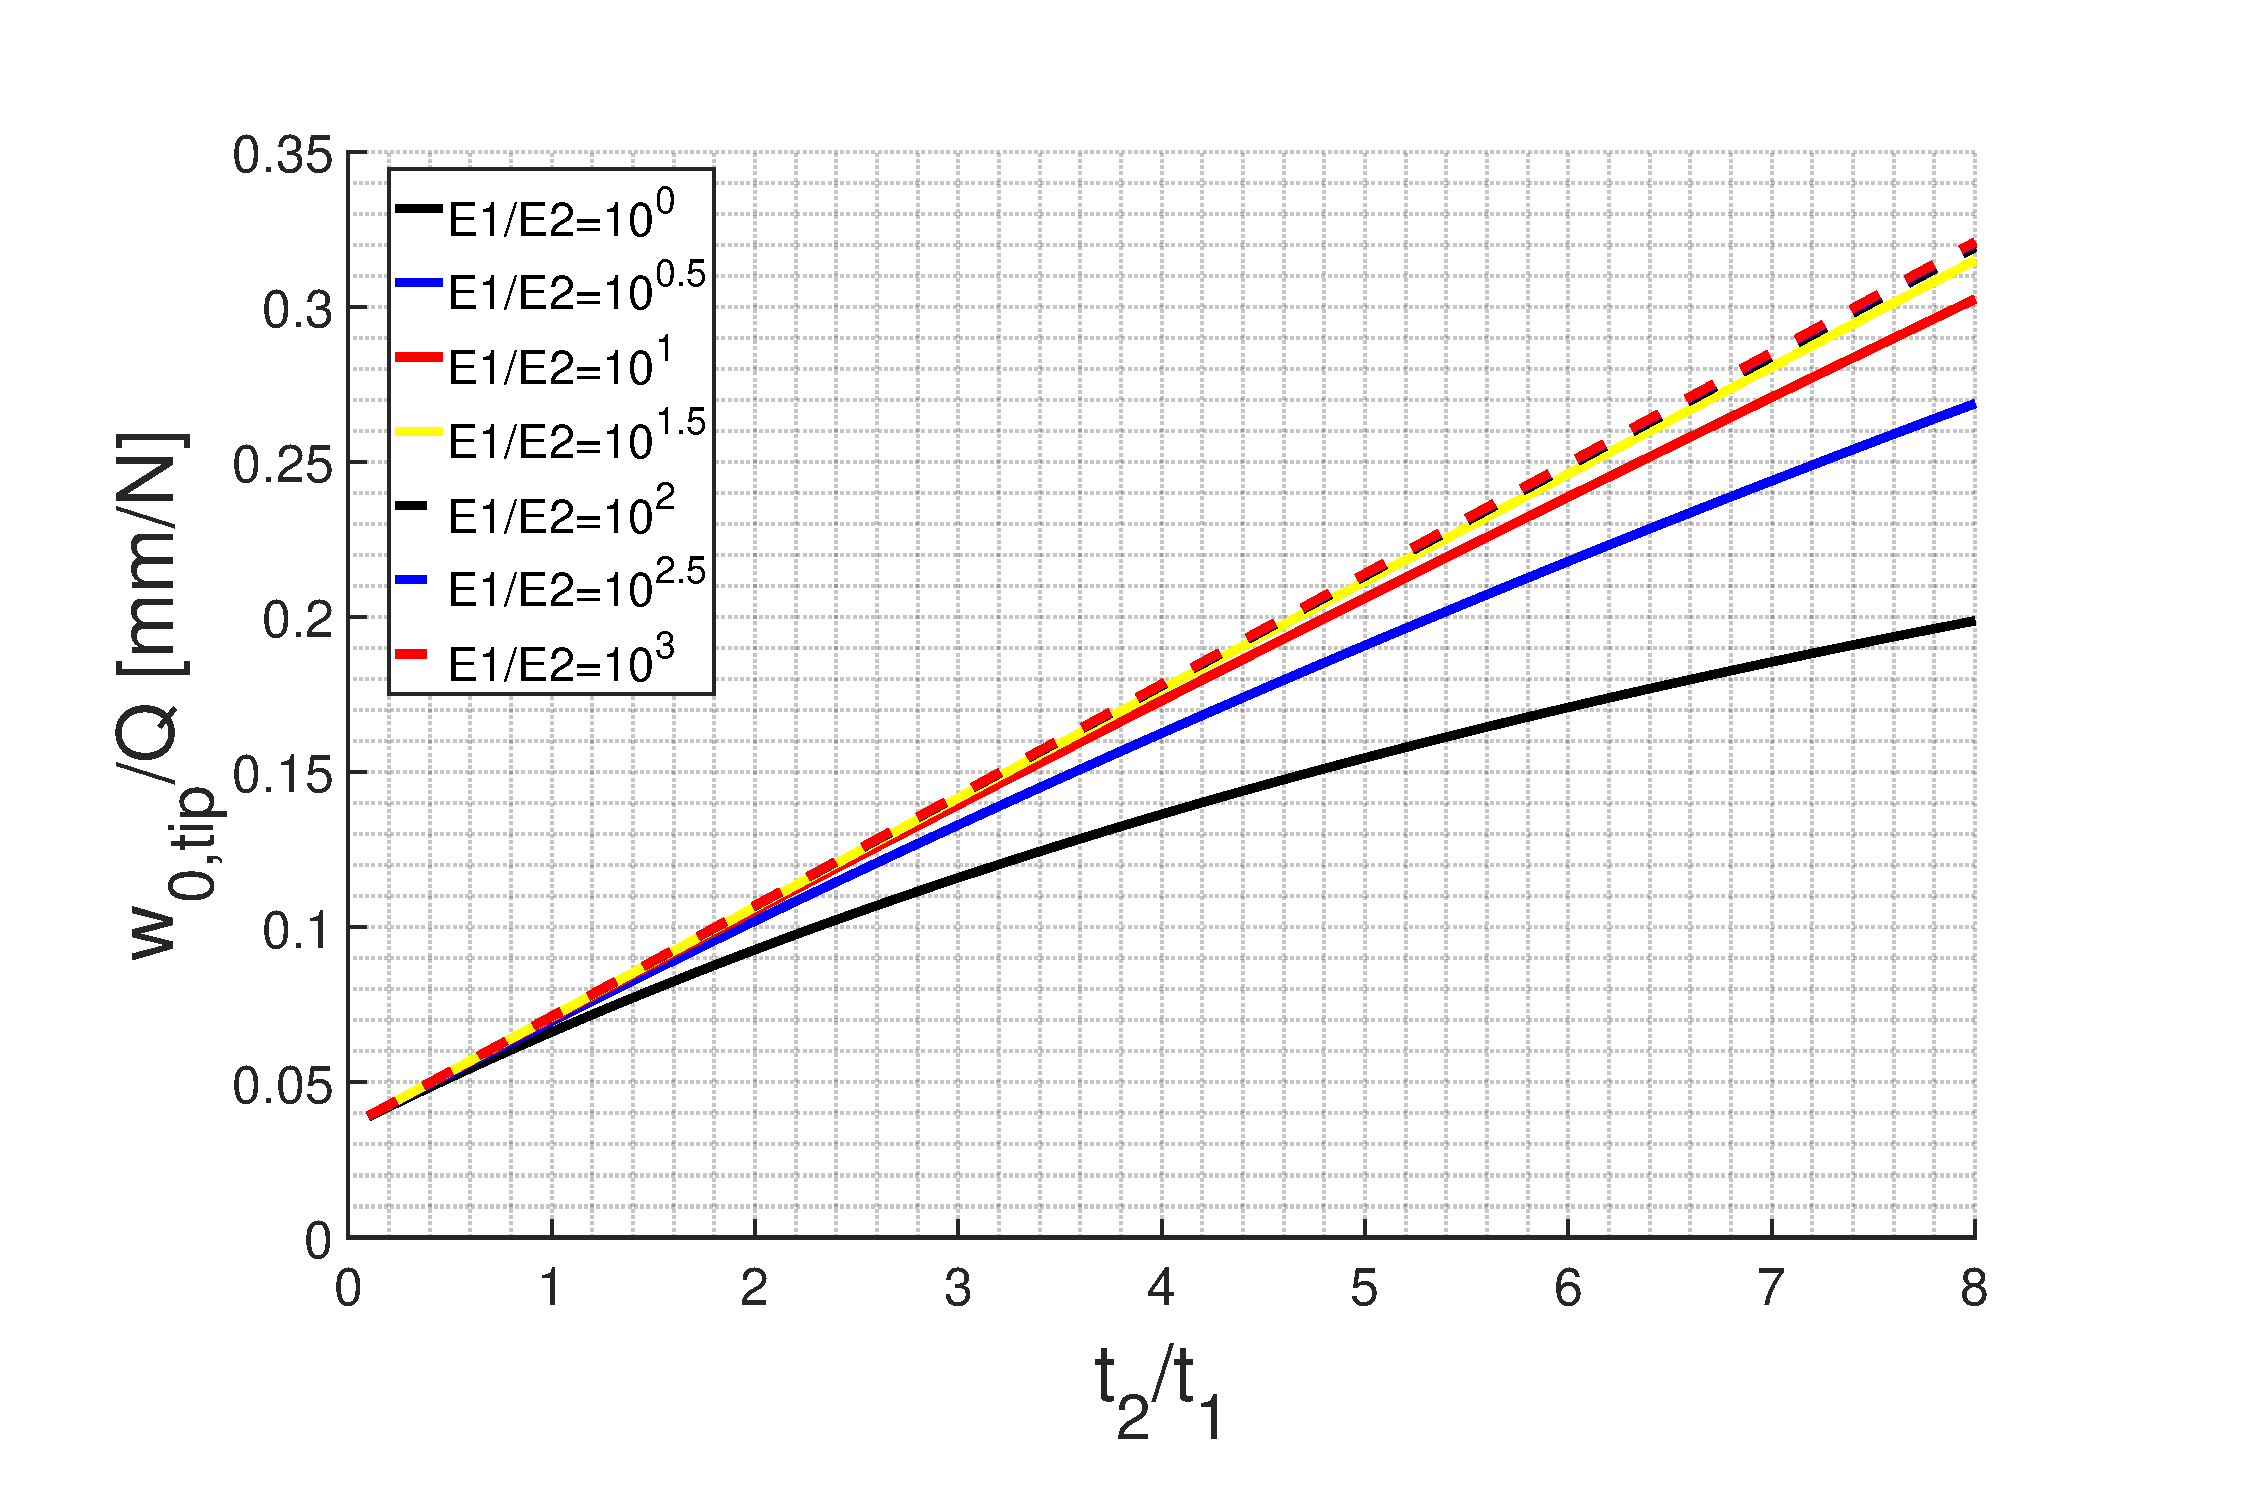
\includegraphics[width=0.8 \textwidth]{../../analytical/figures/woverQ-E1overE2-t2overt1}
  \caption[Influence of the thickness ratio $t2/t1$ on the deflection compliance]{Influence of the thickness ratio $t2/t1$ on the deflection compliance $w_{\mathrm{0,tip}} / Q$ is shown for various values of the stiffness ratio $E_1/E_2$ ranging from $10^0$ to $10^3$. }\label{fig:woverQ-E1overE2-t2overt1}
\end{figure}

\begin{figure}[!htpb] %\phi_tip / Q versus t2/t1, torsional compliance
  \centering
  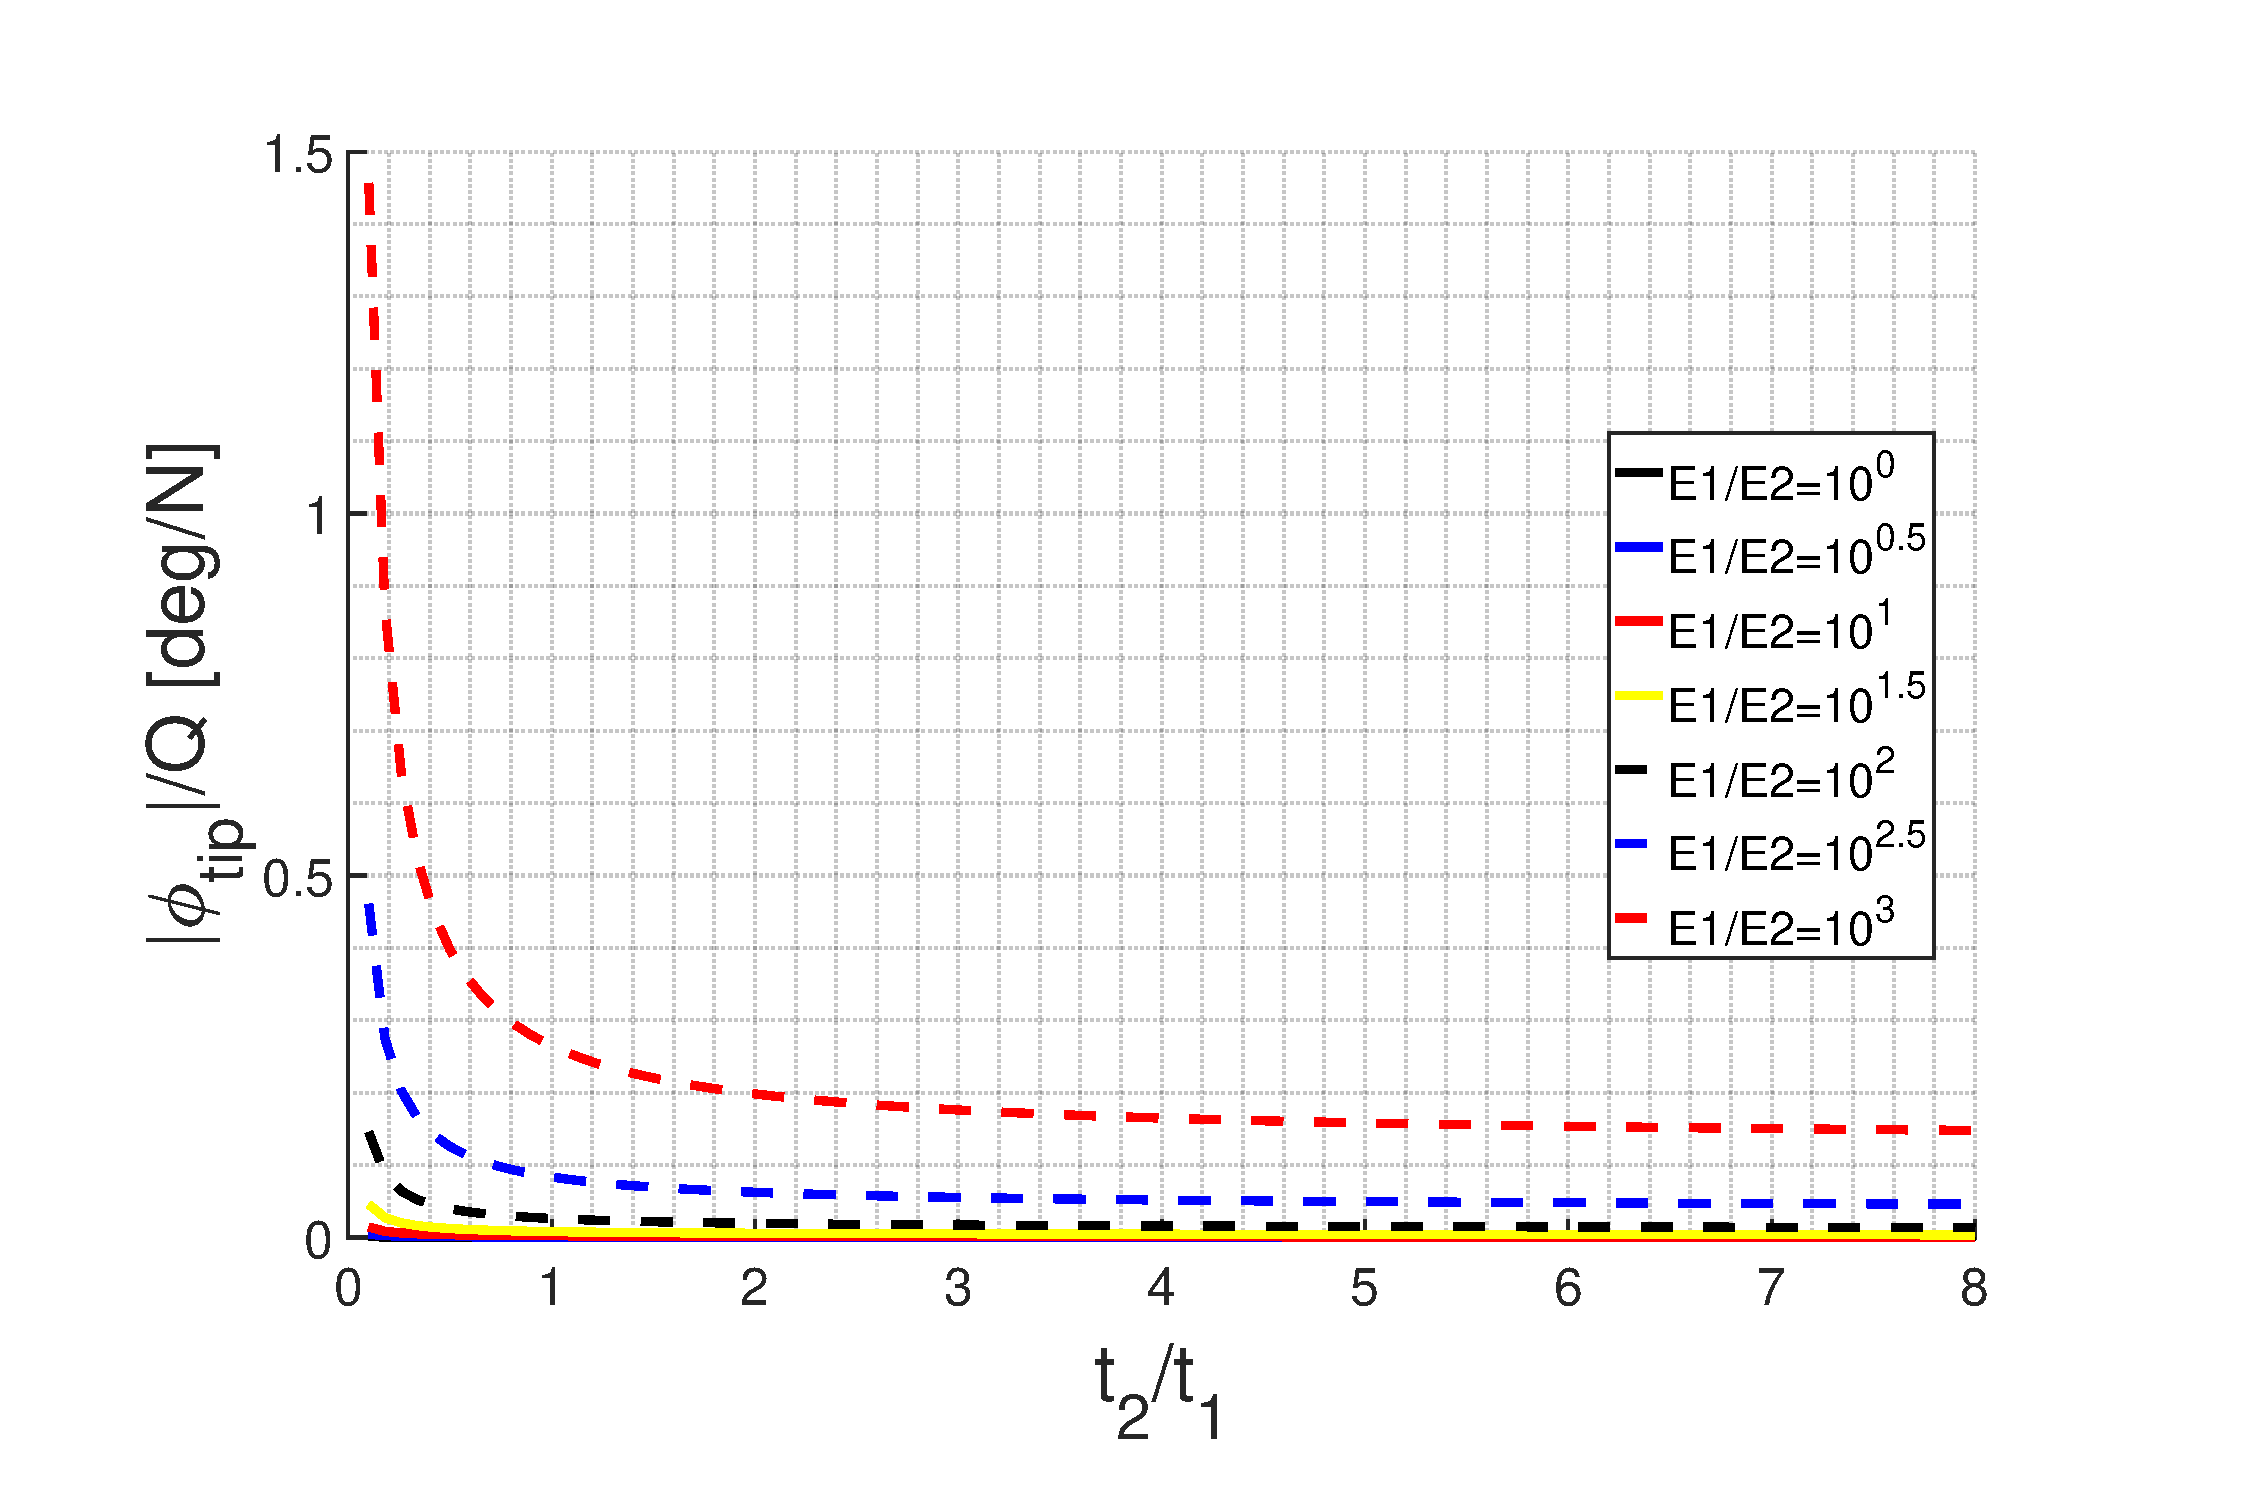
\includegraphics[width=0.8 \textwidth]{../../analytical/figures/phioverQ-E1overE2-t2overt1}
  \caption[Influence of the thickness ratio $t2/t1$ on the torsional compliance]{Influence of the thickness ratio $t2/t1$ on the torsional compliance $|\phi_{\mathrm{tip}}| / Q$ is shown for various values of the stiffness ratio $E_1/E_2$ ranging from $10^0$ to $10^3$. }\label{fig:phioverQ-E1overE2-t2overt1}
\end{figure}

%%%% Figures variation of L / B
\begin{figure}[!htpb] %w_0,tip / Q versus L/B, deflection compliance
  \centering
  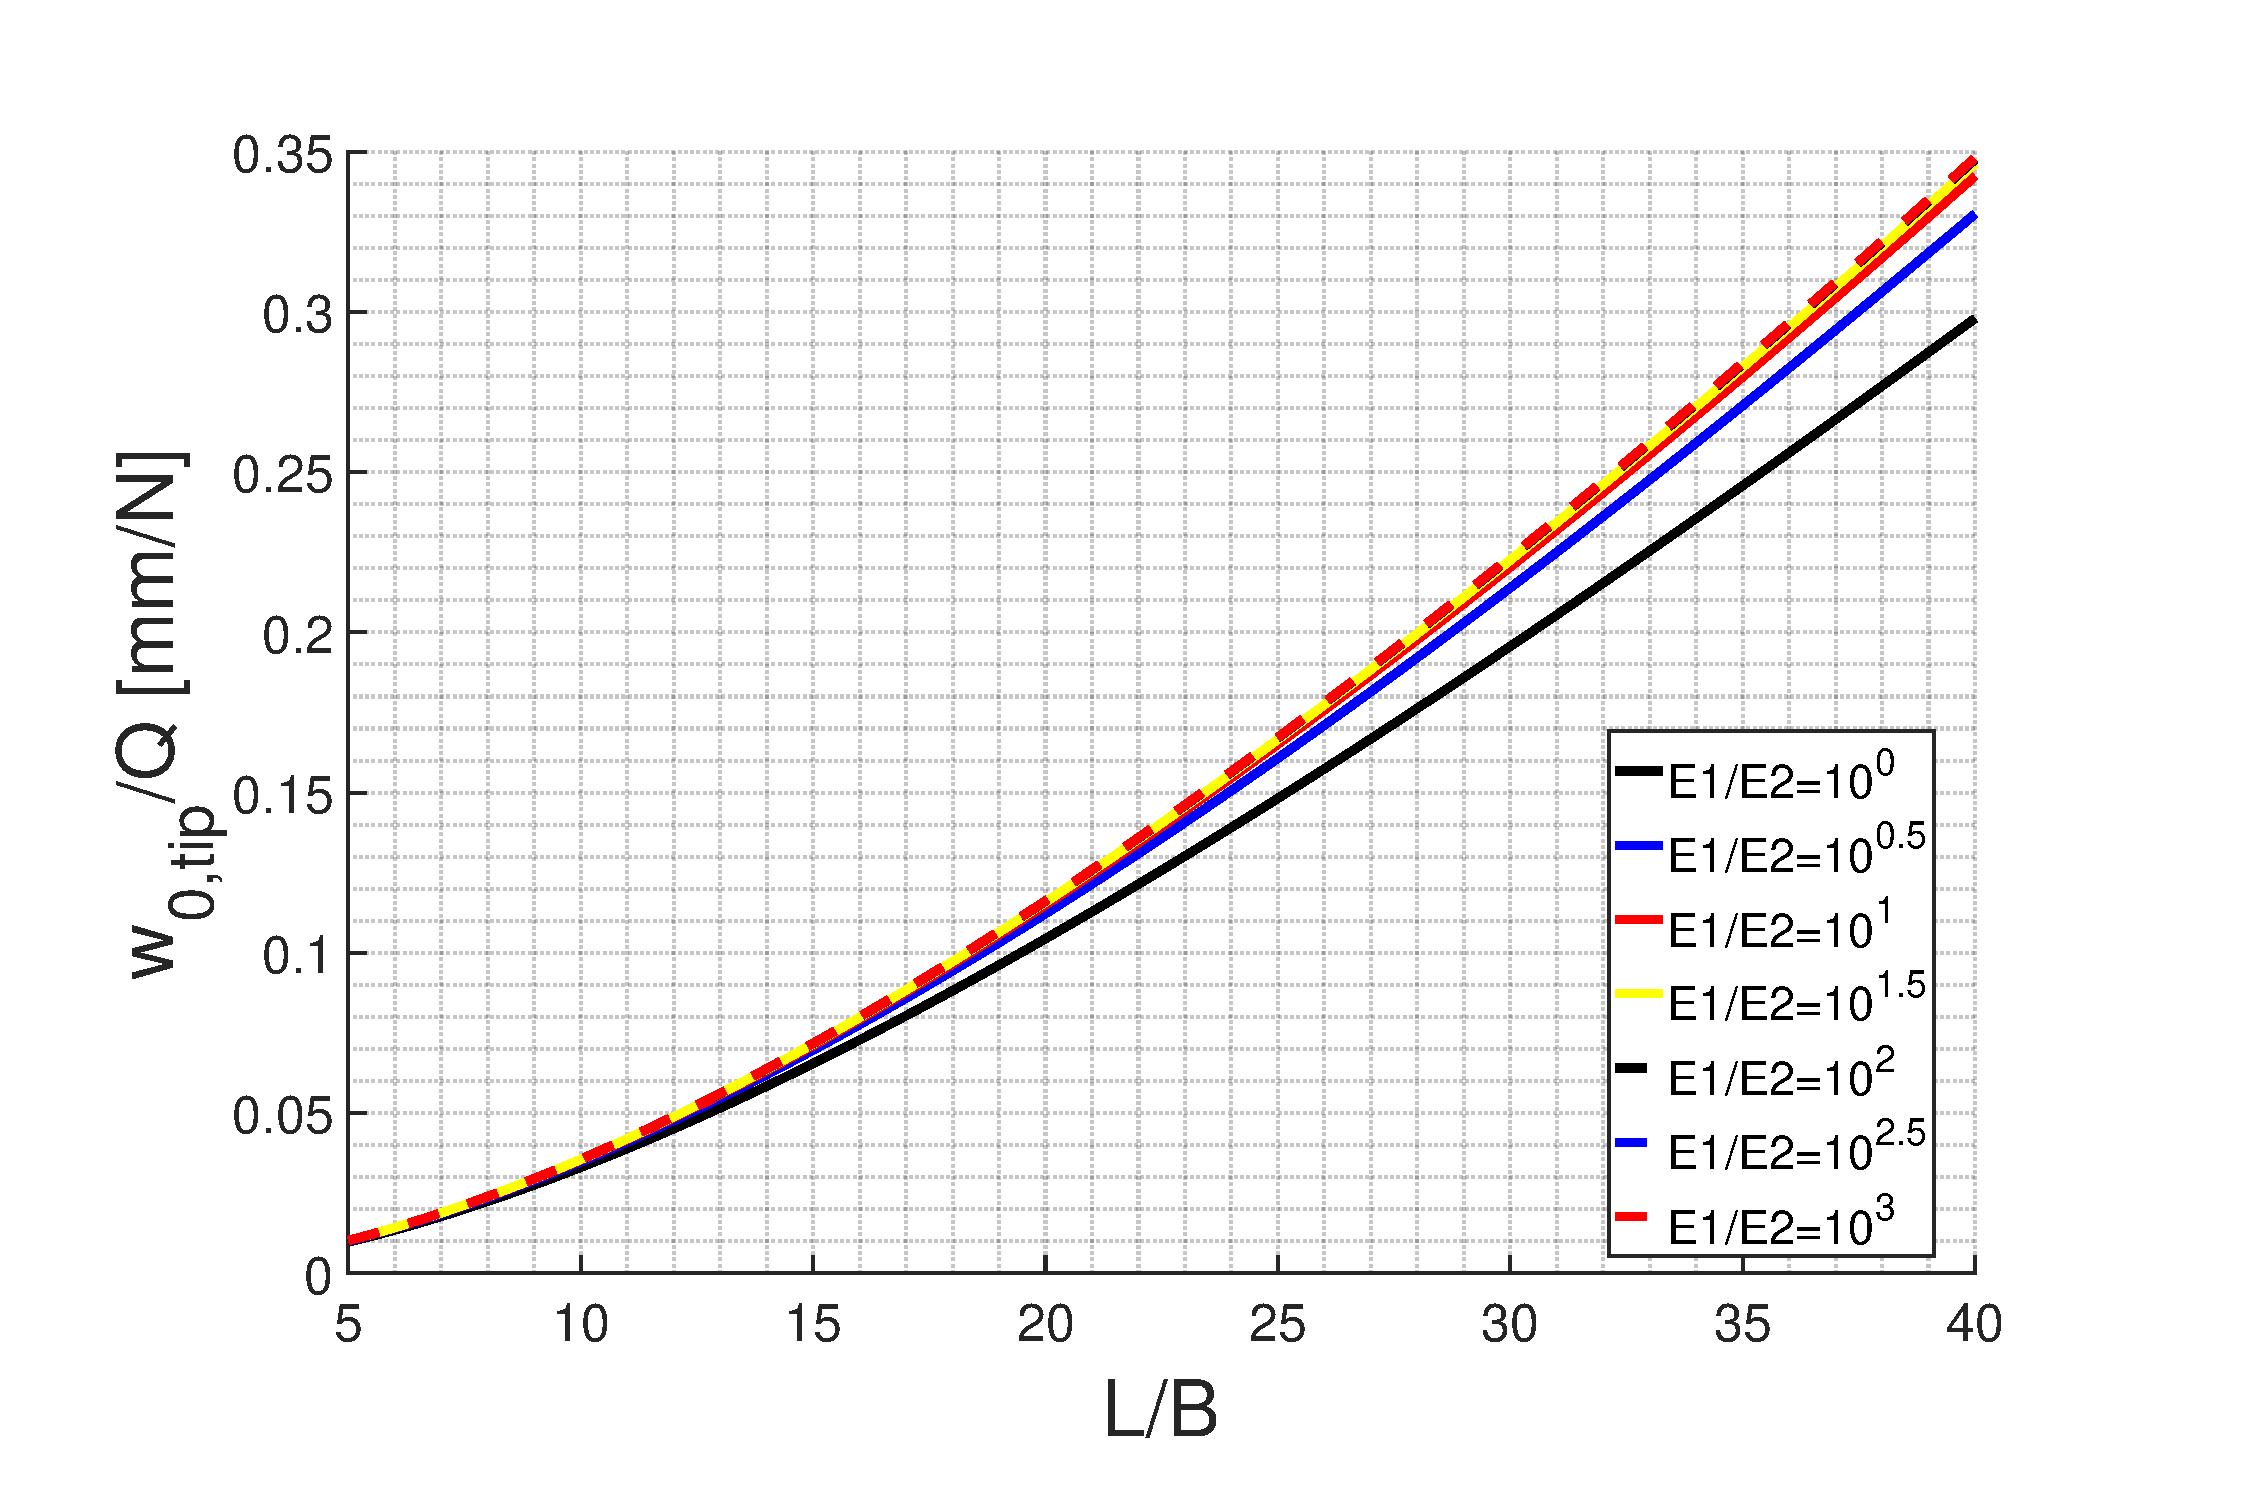
\includegraphics[width=0.8 \textwidth]{../../analytical/figures/woverQ-E1overE2-LoverB}
  \caption[Influence of the slenderness ratio $L/B$ on the deflection compliance]{Influence of the slenderness ratio $L/B$ on the deflection compliance $w_{\mathrm{0,tip}} / Q$ is shown for various values of the stiffness ratio $E_1/E_2$ ranging from $10^0$ to $10^3$. }\label{fig:woverQ-E1overE2-LoverB}
\end{figure}

\begin{figure}[!htpb] %\phi_tip / Q versus L/B, torsional compliance
  \centering
  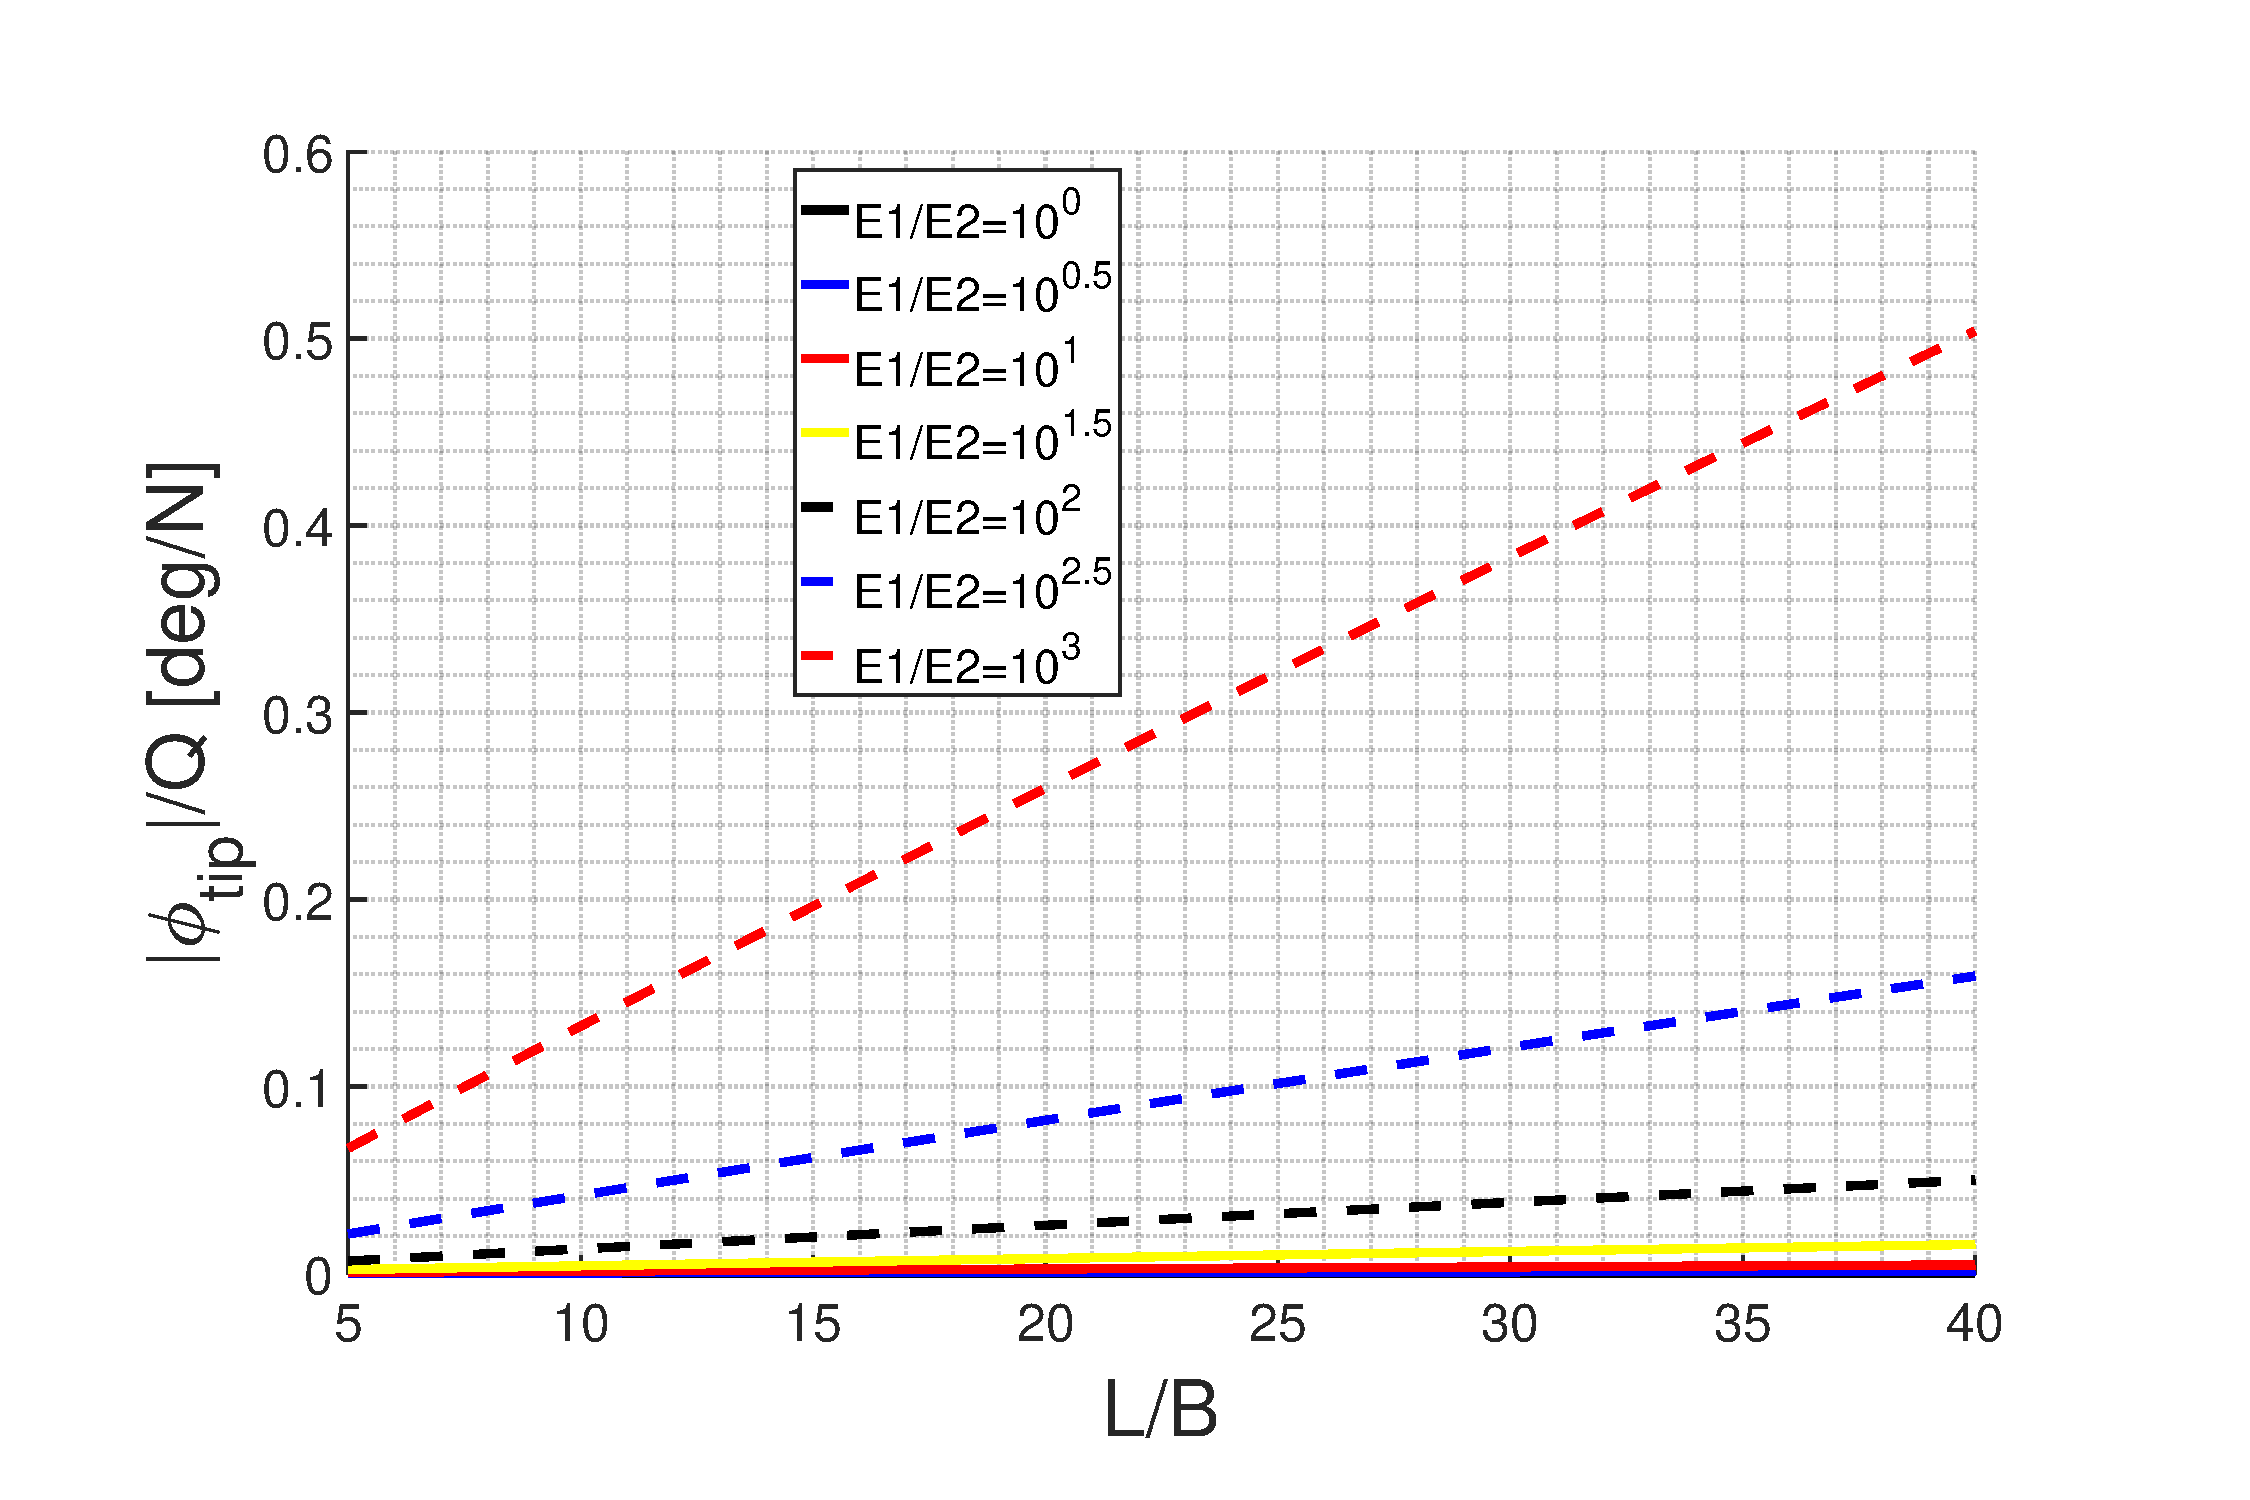
\includegraphics[width=0.8 \textwidth]{../../analytical/figures/phioverQ-E1overE2-LoverB}
  \caption[Influence of the slenderness ratio $L/B$ on the torsional compliance]{Influence of the slenderness ratio $L/B$ on the torsional compliance $|\phi_{\mathrm{tip}}| / Q$ is shown for various values of the stiffness ratio $E_1/E_2$ ranging from $10^0$ to $10^3$. }\label{fig:phioverQ-E1overE2-LoverB}
\end{figure}

\clearpage
\subsection{Discussion of the results} \label{ubsec:disc_results_parametricStudy}

The maximum torsional stiffness $G I_t$ as a function on the cross-sectional aspect ratio $B/H$ can be visualized in Figure \ref{fig:GIt-E1overE2-BoverH}. It can be seen that it appears for $B/H = 1$ when $E_1/E_2 = 1$. Therefore, as it is also shown in \cite{Raither2013a}, the closer the torsional stiffness to the doubly symmetric case, the higher its torsional stiffness. However, when $E_1/E_2 > 10$, the maximum torsional stiffness is shown to appear for $B/H > 1$. A similar conclusion can be extract when analysing the Figure \ref{fig:GIt-E1overE2-t2overt1}, that shows the influence of the thickness ratio $t_2/t_1$ on the torsional stiffness $G I_t$.

In Figure \ref{fig:SC-E1overE2-BoverH} it can be seen that for values $E_2 \ll E_1$, the shear centre position $y_{\mathrm{SC}}$ is approximately constant for $B/H$ variations. In this context, the beam approximates its behavior as if it has an open profile section. However, as the value of $E_1/E_2$ decreases, the influence of the ratio $B/H$ increases showing a bigger influence of the web where the Young's modulus $E_2$ applies. On the other hand, Figure \ref{fig:SC-E1overE2-t2overt1} shows that the bigger the thickness ratio $t_2/t_1$ is, the closer that the shear centre $y_{\mathrm{SC}}$ will be to the vertical axis of simmetry. However, for $E_2 \ll E_1$ the influence of the thickness ratio $t_2/t_1$ is reduced.

The influence of the cross-sectional aspect ratio $B/H$ and the tickness ratio $t_2/t_1$ on the flexural stiffness $E I_y$ is shown to be bigger that that of the Young's modulus ratio $E_1/E_2$, as shown on Figures \ref{fig:EIy-E1overE2-BoverH} and \ref{fig:EIy-E1overE2-t2overt1}, respectively.

% The beam torsional compliance is highly dependant on that torsional moment applied on the beam, that depends on the shear centre $y_{\mathrm{SC}} position. Therefore, as shown on Figure \ref{fig:phioverQ-E1overE2-t2overt1}, the beam's torsional compliance is approximately constant for values of thickness ratio $t_2/t_1 > 1$.

%Comparison of the torsional compliance at the tip against stiffness ratiosub

\section{Computational model analysis} \label{sec:computationalModelAnalysis_results_model}

\subsection{Baseline configuration} \label{subsec:baselineConfig_results_model}

  For this reason, it was decided not to use a model where the connection between the chiral lattice and the wing-box skin is modeled following the approach exposed in the Subsection \label{subsec:connections_computationalModel}. Instead, a more rough connection is used, as shown in Figure \ref{fig:connectionForParametric}.

  \begin{figure}[!htpb]
    \centering
    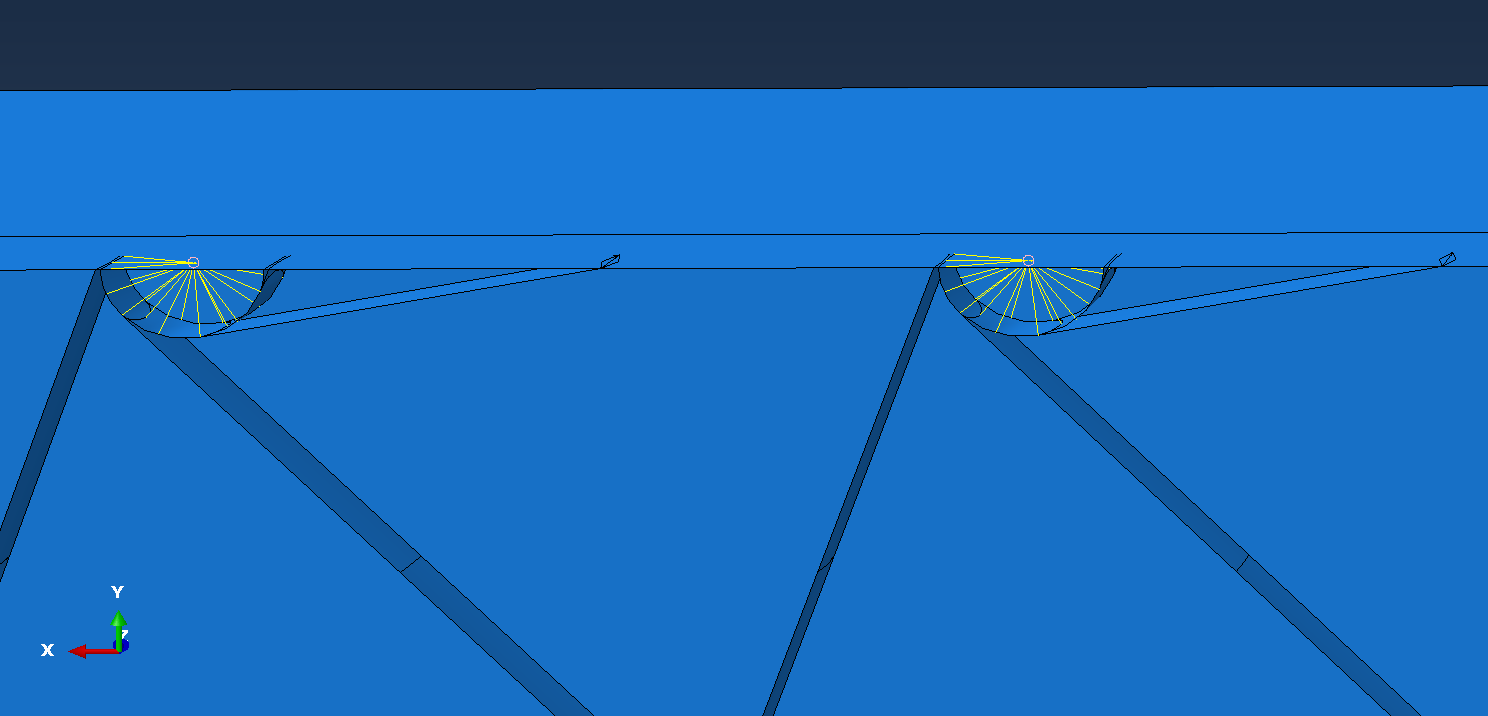
\includegraphics[width=0.8 \textwidth]{result-model/connectionSimple}
    \caption[Connection between the chiral lattice and the wing-box for the parametric study]{Connection between the chiral lattice and the wing-box for the parametric study.}\label{fig:connectionSimple}
  \end{figure}

\subsubsection{Load definition}

\subsubsection{Boundary condition}

  The boundary condition was the one shown in Figure \ref{fig:fixed}. It consisted in a kinematic coupling similar to the introduced in Section \ref{subsec:parametrization_Model} to model the rigid body behavior of the lattice nodes. In this case, the kinematic coupling is establish between a reference point approximately located at the centre of the root rib and the faces of this mentioned rib. The reference point acts as a master node while the mesh nodes located at the faces of the rib are the slave nodes. The reference point is next fixed in all its degrees of freedom using the corresponding boundary condition Abaqus module.

  \begin{figure}[!htpb]
    \centering
    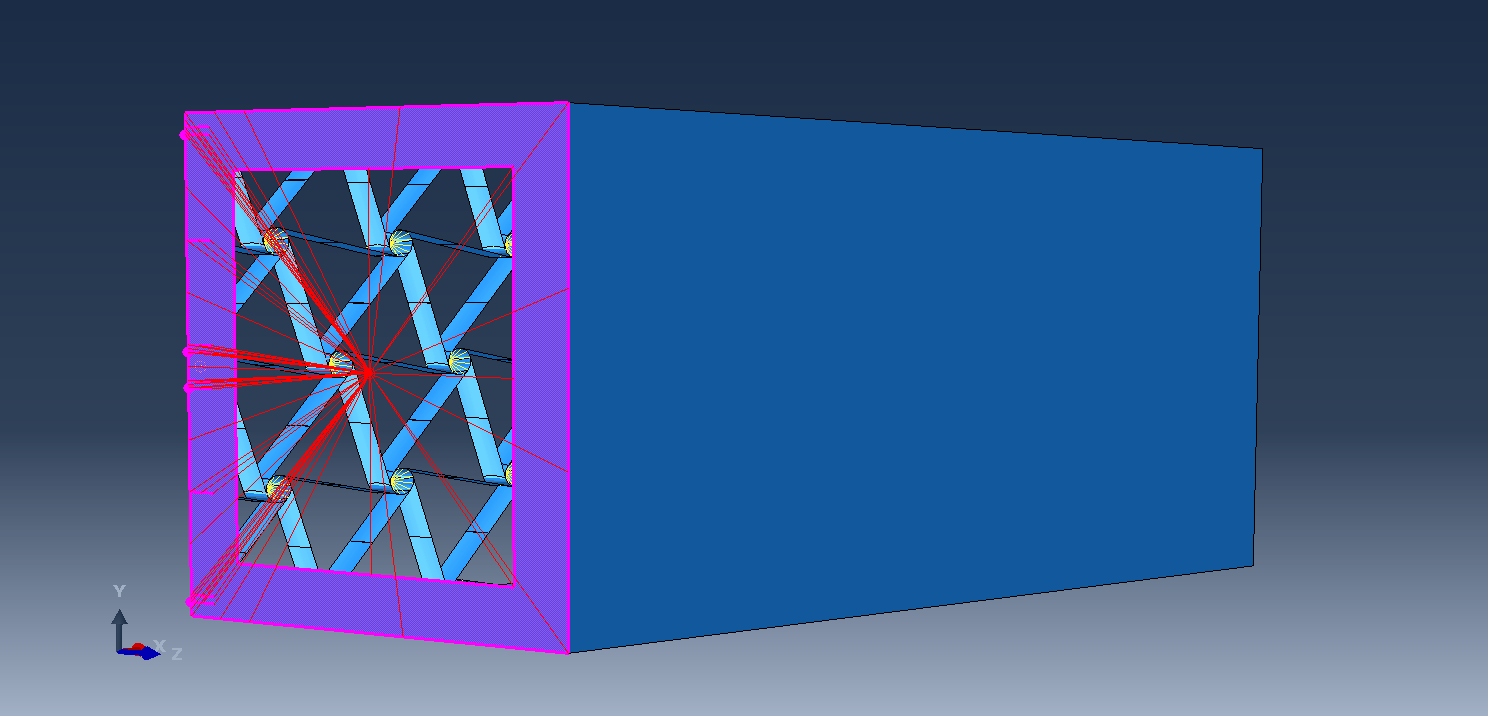
\includegraphics[width=0.8 \textwidth]{../figures/result-model/fixed}
    \caption[Boundary condition for the model]{Boundary condition for the model. The condition is establish through a coupling interaction between a reference point and the faces of the rib at the root. The reference point is next fixed in all its degrees of freedom using the corresponding boundary condition Abaqus module.}\label{fig:fixed}
  \end{figure}

\subsubsection{Results analysis} %To be extended, maybe

  The results obtained from the Abaqus simulations were analyzed in two different ways. Firstly, qualitatively by means of the deformation plots that shown by the Abaqus. And, secondly, extracting values of different magnitudes directly from the mesh nodes or elements located at certain positions of interest.

  Through the definition of paths in Abaqus, it is possible to obtain the value of a determined magnitude for all the mesh elements located along the path. In Figure \ref{fig:pathUpper}, an example of a path located on the upper skin of the wing-box is shown.

  \begin{figure}[!htpb]
    \centering
    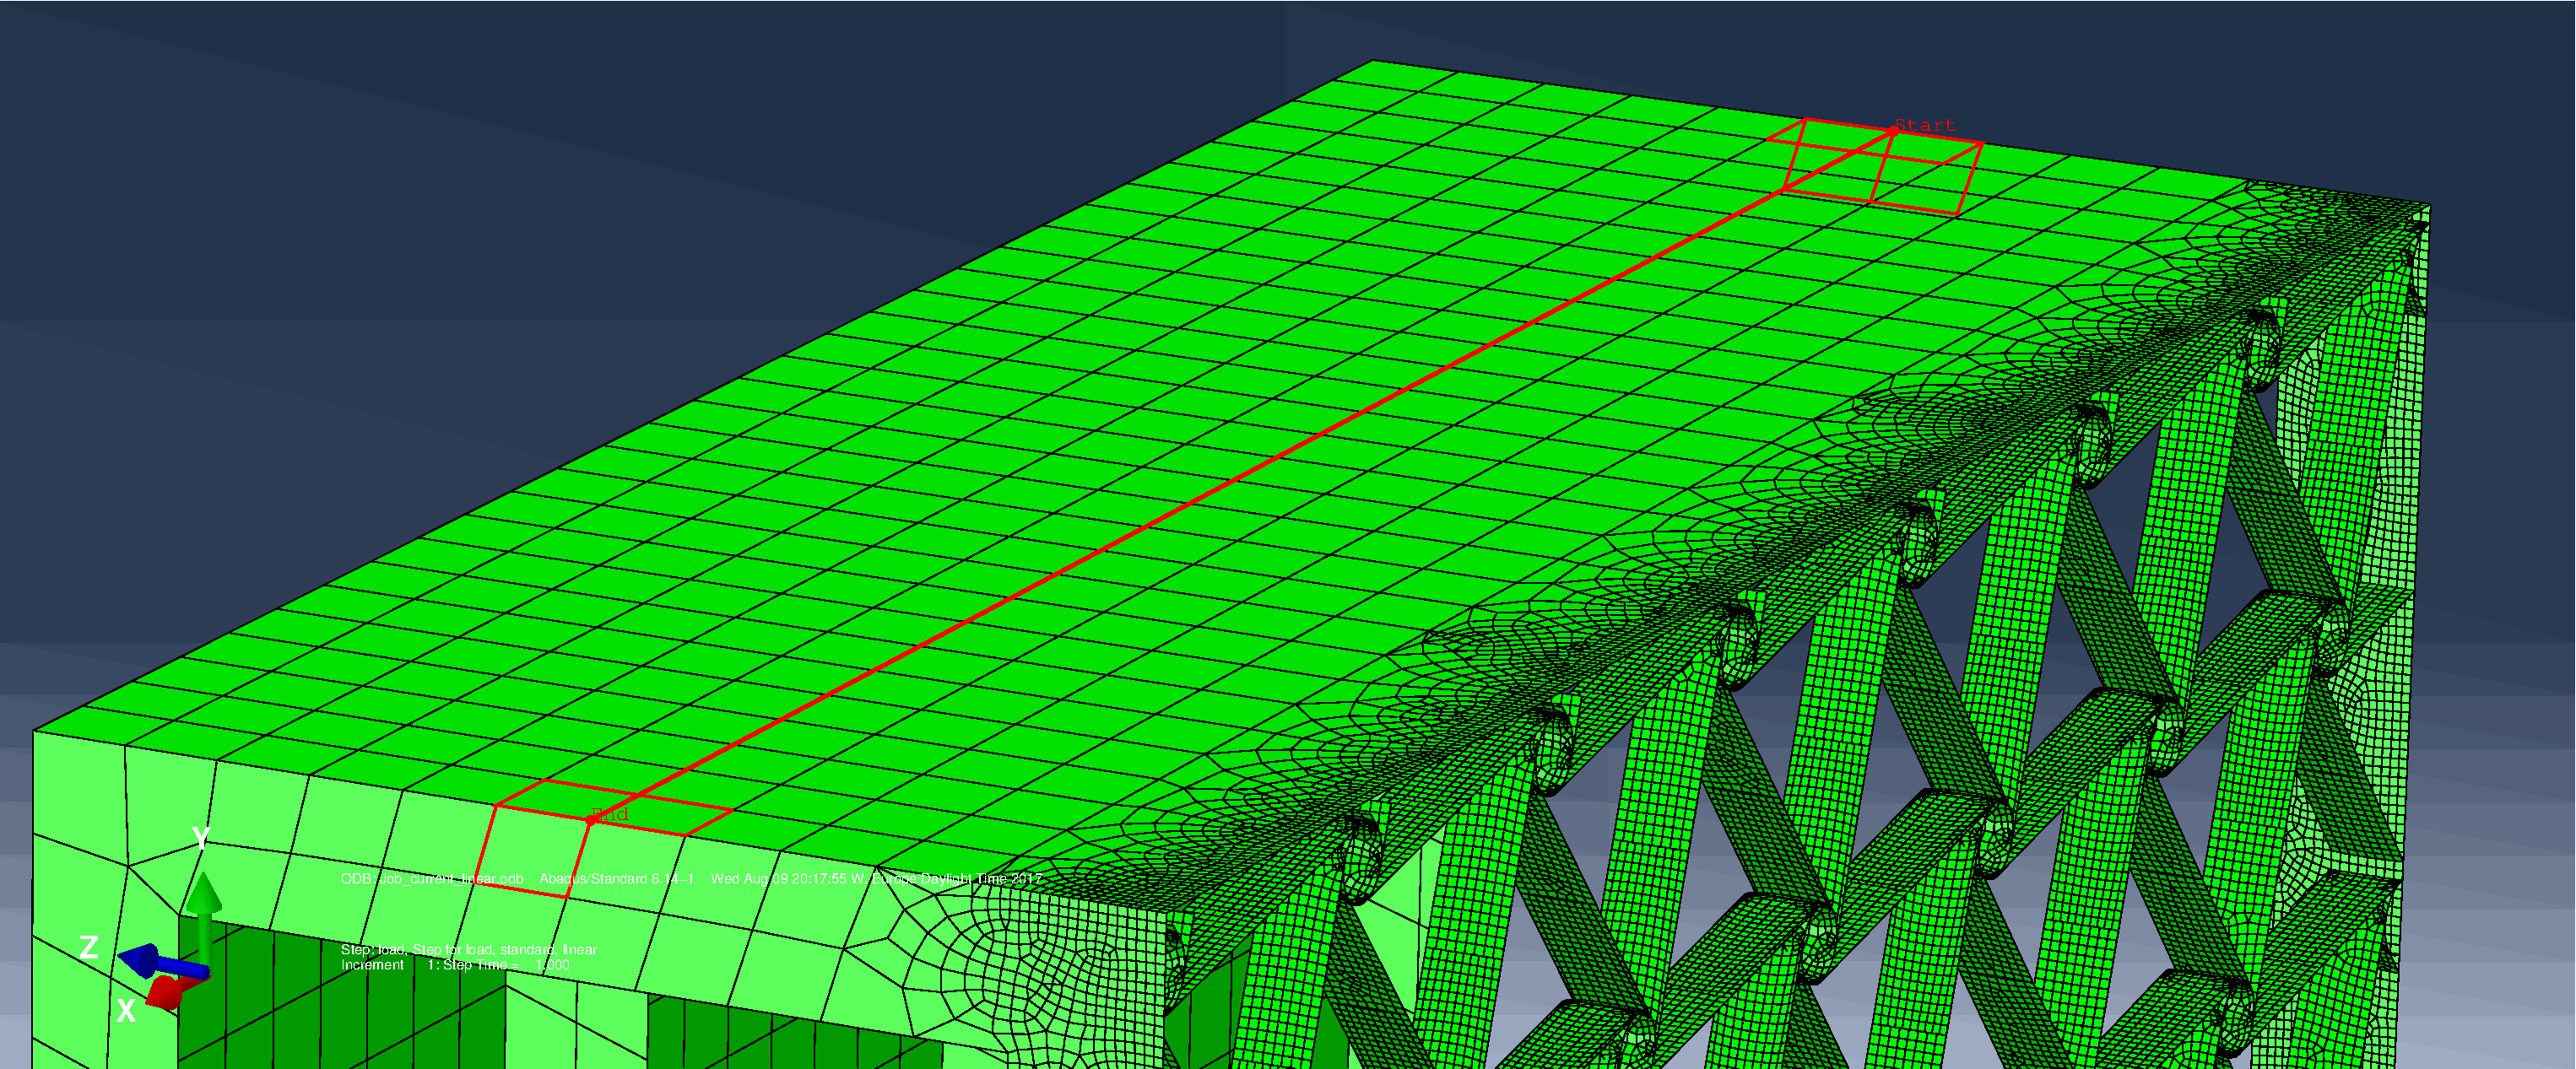
\includegraphics[width=0.8 \textwidth]{../figures/result-model/pathUpper}
    \caption[Path of mesh elements on the solution model]{Path of mesh elements on the solution model.}\label{fig:pathUpper}
  \end{figure}

\subsubsection{Nonlinear problem and automatic stabilization} %TO BE REVIEWED
  
  For the case under study, nonlinear simulations will be carried out as is expected to find a nonlinear load-displacement curve as a result of the analysis. In Abaqus, to execute nonlinear simulation involves the following, as shown in \cite{Abaqus}:

  \begin{itemize}
    \item a combination of incremental and iterative procedures;
    \item using the Newton method to solve the nonlinear equations;
    \item determining convergence;
    \item defining loads as a function of time; and
    \item choosing suitable time increments automatically.
  \end{itemize}

  Therefore, Abaqus breaks the step where the load is applied into increments. The software will automatically choose the size of each of the increments based on the convergence evolution of previous increments.

  Also, nonlinear static problems may become unstable. One of the possible sources of such instabilities is buckling. A model where buckling appears locally may not be resoluble using general solution methods. For this kind of cases, it becomes necessary to either solve the problem dynamically or with the aid of artificial damping.

  Since the above situation represents what it is expected to be found in the model response, a constant artificial damping factor will be used throughout the whole step to account for the appearance of local instabilities.  

  Automatic stabilization with a constant damping factor implies that viscous forces of the form
  $$
  F_v = c \mat{M} v
  $$
  are added to the global equilibrium equations
  $$
  P - I - F_v = 0,
  $$
  where $I$ represents the internal forces, $P$ the external forces, $\mat{M}$ is the artificial mass matrix calculated with unity density, $c$ is the defined damping factor, $v = \Delta u / \Delta t$ is the vector of nodal velocities, and $\Delta t$ is the increment of simulation time.

  For the simulations run, a damping factor of the order of $\approx$10$^{-8}$ was found to be sufficient for the simulations to achieve convergence.

\section{General response characterization} \label{sec:generalResponseCharact}

  %Figure XX: Path on upper flange of wing-box

  %Solution characterization
  % -> For the normal case
  %     - \ref{fig:normalCaseNoDampNoInnerRibs_800N}
  %     - the initial buckling ocurrs far from the root
  %     - UR1 of ~0.3 deg at the beam tip
  %
  % -> Introduccing damping
  %     - \ref{fig:normalCaseNoDampNoInnerRibs_800N}
  %     - Really big local deformations appear on the wing-box upper surface
  %     - UR1 of one order of magnitude higher, 3deg at the tip
  %     - Introduccing inner ribs becomes necessary to achieve greater twist with reduced local deformation
  %     - There is a point at which the structure collapses
  %     - \ref{fig:normalCaseDampNoInnerRibs_800N}
  %     - See plot that compares the external work introduced in the system and the static energy dissipated through artificial stabilization. \ref{fig:normalCaseNoDampNoInnerRibs_800N_stabilizationPlot}
  %
  % -> Introducing inner ribs but not damping
  %     - \ref{fig:normalCaseNoDamp2InnerRibs_800N}
  %     - Buckling again appears at the front at it is very little
  %     - The simulation stops really soon, only tau/T = 0.134 achieved for the current plot
  % -> Introducing damping and inner ribs 
  %     - Twist at the tip is now of about 0.68deg
  %     - The energy plot for this is \ref{fig:normalCaseDamp2InnerRibs_800N_stabilizationPLot}
  %     - The deformation plot shows now how buclking start at the lattice located close to the inner rib more close to the root, in a positive x from the position of the rib. The buckling then moves a group of lattices at the root, in the upper position of the lattice.
  %     - Some local deformation still ocurrs at the section of the wing-box skin located in between the root at the first inner rib.
  %     - However, the inner ribs help the upper skin of the wing-box to remain more flat than before.

\subsection{Connection between the chiral lattice and the wing-box skin} \label{subsec:connection_results_model}


\subsection{Connection between the chiral lattice and the wing-box skin} \label{subsec:connection_results_model}

Two different approaches were followed to model the rigid body behavior of the lattice nodes, as shown in Section \ref{subsec:parametrization_Model}.

The modeling of the lattice nodes through either the coupling through a reference point and through tyre was shown to 

\subsection{Mesh} \label{subsec:mesh_results_model}

The model was build using cell shell elements as the fundamental constituting part. The thickness is assigned in the perpendicular direction, as it was shown in Figure \ref{fig:shellElement}.

This type of element is a 2D element that it was used to build 3D structures. This kind of procedure may incur some distortion in the mesh elements due to shell elements intersecting in the same line at different angles. 

For the designed model, this situation occurred at the chiral lattice at certain points. As soon in Figure \ref{fig:meshDistorted} it can be seen that the distorted elements appear at mainly at two different positions. Firstly, at the plane where the two ligaments with different curvature join. At this point, the sharp angles that appear in between the part geometrical lines induce the appearance of tetrahedral distorted mesh elements. The second typical location for appearance of distorted elements is along the curve where the lattice nodes and the curved ligaments join.

\begin{figure}[!htpb]
  \centering
  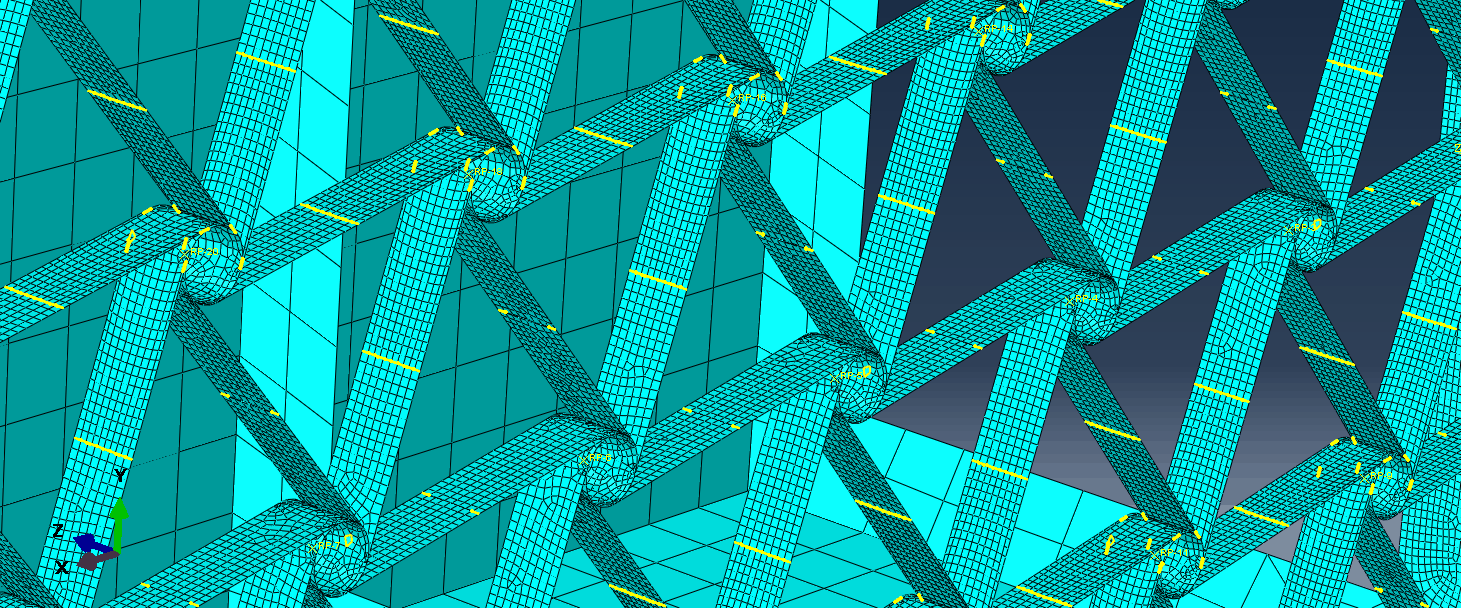
\includegraphics[width=0.8 \textwidth]{result-model/meshDistorted}
  \caption[Distorted mesh elements in the model]{Distorted mesh elements in the model. The number of distorted elements was found to be crucial for the simulation convergence.}\label{fig:meshDistorted}
\end{figure}

It was seen that the number of distorted elements had a significant effect in the simulation convergence. For a high number of distorted elements, the simulation could not go further from the first step. No attempts to locally modify the mesh at the mentioned locations were made, instead, it was found that modifying the global mesh size gave enough control over the number of distorted elements to be able to overcome this limitation. The bigger the mesh size in the area, the less distorted elements appear after completing the meshing operations.
